\documentclass[10pt]{article}
\usepackage{kotex}
\usepackage{amssymb}
\usepackage{amsmath}
\usepackage{graphicx}
\usepackage{subfigure}
\usepackage{booktabs}
\usepackage{multirow}
\usepackage{titlesec}
\usepackage[hidelinks]{hyperref}

\titleformat{\section}
  {\normalfont\large\sffamily\bfseries}
  {\thesection.}
  {1em}
  {}
\titleformat{\subsection}
  {\normalfont\normalsize\sffamily\bfseries}
  {\thesubsection}
  {1em}
  {}

\renewcommand{\thesection}{\arabic{section}}
\renewcommand{\thesubsection}{\thesection.\arabic{subsection}}

\usepackage{setspace}
\setstretch{1.31}

\textwidth 17.6cm
\textheight 24.2cm
\addtolength{\oddsidemargin}{-25mm}
\addtolength{\topmargin}{-21mm}
\setcounter{page}{0}

\newcommand{\figwidth}{12.4cm}
\newcommand{\smallfigwidth}{10.8cm}

\begin{document}

\begin{center}
{\LARGE \bf 잡음 비디오의 저비트레이트 H.264 인코딩을 위한 3차원 DT-CWT 전처리의 조건부 성능 분석}\\[12pt]
민찬, 지도교사\\
서울과학고등학교\\[12pt]
{\LARGE \bf Conditional Performance Analysis of 3D DT-CWT Preprocessing for Low-Bitrate H.264 Encoding of Noisy Video}\\[12pt]
Minchan, Advisor\\
Seoul Science High School\\[12pt]

{\large \bf 국문 초록}
\noindent\rule{\textwidth}{0.4pt}
\begin{flushleft}
본 연구는 잡음이 포함된 비디오를 저비트레이트 H.264/x264로 인코딩하기 전에 3차원 dual-tree complex wavelet transform(3D DT-CWT) 전처리를 적용했을 때의 조건부 성능을 분석하였다. 일반적인 영상 전처리 연구는 전처리 후 영상이 원본에 얼마나 가까워졌는지를 주로 평가하지만, 실제 전송 및 저장 환경에서는 전처리 결과가 코덱을 통과한 뒤에도 rate--distortion(RD) 성능 개선으로 이어지는지가 더 중요하다. 이를 확인하기 위해 CIF 해상도의 \textit{akiyo}, \textit{foreman}, \textit{mobile}, \textit{stefan} 네 영상을 사용하고, 휘도 채널에 Gaussian 잡음 $\sigma=0,5,10,15$를 추가한 뒤 100--500 kbps에서 x264 인코딩을 수행하였다. 제안 방법은 전처리 없는 x264 baseline, x264 내부 noise reduction, FFmpeg hqdn3d, 3D DWT, Gaussian blur와 비교하였다. 평가는 PSNR만이 아니라 저비트레이트 코덱에서 중요한 블로킹 왜곡을 반영하는 PSNR-B와 GBIM, 구조 유사도를 반영하는 MS-SSIM, 시간적 통계 차이를 반영하는 STRRED-like score를 함께 사용하였다. 본 논문의 delta는 모두 \textit{Proposed - Baseline}으로 정의하였다. 실험 결과, clean 영상에서는 제안 방법이 평균 PSNR 기준으로 약 0.08 dB 감소하여 전처리 오버헤드가 확인되었다. 반면 noisy 조건 전체에서는 평균 0.71 dB의 PSNR 이득과 0.90 dB의 PSNR-B 이득, 0.0088의 MS-SSIM 이득을 보였으며, GBIM은 모든 noisy 조건에서 감소하였다. 특히 저움직임 영상인 \textit{akiyo}에서는 $\sigma=15$에서 평균 PSNR 2.87 dB, PSNR-B 3.87 dB, MS-SSIM 0.036의 큰 개선이 나타났고, GBIM과 STRRED-like score도 각각 -2.22, -0.90으로 감소하였다. 그러나 STRRED-like score는 \textit{akiyo}를 제외한 영상에서 증가하여, 시간적 품질은 영상 움직임에 민감함을 보였다. 또한 pre-x264 전처리 이득보다 post-x264 이득이 작아 codec gain은 대부분 음수로 나타났다. 따라서 본 연구는 3D DT-CWT 전처리가 모든 영상에 보편적으로 우수한 방법이라기보다, \textbf{잡음이 충분하고 움직임이 비교적 안정적인 저비트레이트 조건에서 선택적으로 적용할 때 유효한 전처리}임을 보인다.

\textbf{주제어:} 3D DT-CWT, 비디오 전처리, H.264, 저비트레이트 인코딩, 잡음 제거
\noindent\rule{\textwidth}{0.4pt}
\end{flushleft}

{\large \bf Abstract}
\noindent\rule{\textwidth}{0.4pt}
\begin{flushleft}
This study analyzes the conditional performance of three-dimensional dual-tree complex wavelet transform (3D DT-CWT) preprocessing before low-bitrate H.264/x264 encoding of noisy video. While conventional preprocessing studies often evaluate denoising quality before compression, practical video systems require that preprocessing gains remain meaningful after rate--distortion encoding. Four CIF sequences, \textit{akiyo}, \textit{foreman}, \textit{mobile}, and \textit{stefan}, were corrupted by luma-channel Gaussian noise at $\sigma=0,5,10,15$ and encoded by x264 at 100--500 kbps. The proposed method was compared with direct x264 encoding, x264 noise reduction, FFmpeg hqdn3d, 3D DWT, and Gaussian blur. In addition to PSNR, the evaluation emphasizes PSNR-B and GBIM for blocking artifacts, MS-SSIM for structural similarity, and a STRRED-like score for spatio-temporal statistics. All deltas in this paper are defined as Proposed - Baseline. On clean inputs, the proposed method showed a small average PSNR loss of about 0.08 dB. Across noisy conditions, it achieved an average gain of 0.71 dB in PSNR, 0.90 dB in PSNR-B, and 0.0088 in MS-SSIM, while GBIM decreased in all noisy conditions. The low-motion \textit{akiyo} sequence showed the largest improvement at $\sigma=15$, reaching 2.87 dB in PSNR, 3.87 dB in PSNR-B, 0.036 in MS-SSIM, -2.22 in GBIM, and -0.90 in STRRED-like score. However, the STRRED-like score increased except for \textit{akiyo}, indicating that temporal quality remains sensitive to motion. The measured post-encoding gain was also smaller than the pre-encoding denoising gain, resulting in mostly negative codec gain. These results indicate that 3D DT-CWT preprocessing is not universally beneficial, but is effective when applied selectively to sufficiently noisy and relatively stable low-bitrate video.

\textbf{Keywords:} 3D DT-CWT, video preprocessing, H.264, low-bitrate encoding, denoising
\noindent\rule{\textwidth}{0.4pt}
\end{flushleft}
\end{center}

\section{\large \bf 서론(Introduction)}
디지털 비디오는 저장 공간과 전송 대역폭의 제약 때문에 대부분 손실 압축 과정을 거친다. H.264/AVC와 그 구현체인 x264는 높은 압축 효율 때문에 널리 사용되지만, 목표 비트레이트가 낮아질수록 영상의 세부 구조가 강하게 양자화되고 블록 단위 압축 아티팩트가 증가한다. 이때 입력 영상에 존재하는 센서 잡음이나 저조도 잡음은 장면의 의미 있는 구조와 달리 예측이 어렵고, 프레임 간 상관성도 낮기 때문에 코덱의 비트 예산을 불필요하게 소비한다. 따라서 저비트레이트 인코딩 전에 잡음을 줄이는 전처리는 압축 효율을 높일 수 있는 직관적인 접근이다.

그러나 전처리를 무조건 적용하는 것은 위험하다. 영상의 고주파 성분에는 잡음뿐 아니라 윤곽, 질감, 작은 움직임과 같은 실제 정보도 포함된다. 전처리 필터가 이 성분을 과도하게 줄이면, 깨끗한 영상에서는 오히려 품질이 낮아질 수 있다. 또한 전처리로 얻은 denoising 이득이 x264의 예측, 변환, 양자화 과정을 통과한 뒤에도 동일하게 유지된다는 보장도 없다. 즉 본 연구에서 중요한 질문은 ``전처리 영상이 더 깨끗해졌는가''가 아니라, \textbf{전처리 이후 최종 인코딩 결과가 같은 비트레이트에서 더 좋은가}이다.

본 연구는 이러한 문제의식에서 출발하여 3D DT-CWT 기반 전처리의 성능을 clean/noisy 조건, 낮은/높은 잡음 조건, 낮은/높은 움직임 조건으로 나누어 분석하였다. 연구의 목적은 3D DT-CWT가 기존 전처리보다 항상 우수하다는 주장을 세우는 것이 아니라, \textit{어떤 조건에서 이득이 나타나고 어떤 조건에서 제한되는지}를 실험적으로 밝히는 것이다. 이를 통해 저비트레이트 비디오 인코딩에서 전처리 알고리즘을 선택적으로 적용하기 위한 근거를 마련하고자 한다.

\section{\large \bf 이론적 배경(Theory \& Principle)}
\subsection{저비트레이트 H.264/x264 인코딩}
H.264/AVC는 화면 내 예측, 화면 간 예측, 블록 변환, 양자화, 엔트로피 부호화를 결합한 대표적인 비디오 압축 표준이다[1]. x264는 H.264의 공개 구현체로, 동일한 표준 안에서 실용적인 rate control과 여러 압축 옵션을 제공한다. 저비트레이트 조건에서는 주어진 비트 예산이 작기 때문에 인코더가 더 강한 양자화를 수행하며, 그 결과 고주파 성분과 작은 움직임이 손실되기 쉽다.

잡음은 압축에서 두 가지 문제를 일으킨다. 첫째, 잡음은 공간적으로 불규칙하여 변환 계수의 에너지를 넓게 퍼뜨린다. 둘째, 잡음은 시간적으로도 안정적인 예측이 어렵기 때문에 움직임 보상으로 제거되기 어렵다. 따라서 noisy 입력에서는 동일한 목표 비트레이트에서도 clean 입력보다 실제 장면 구조가 더 많이 손상될 수 있다. 이 연구에서 전처리는 이러한 잡음 성분을 인코딩 전에 줄여 x264가 장면 구조에 더 많은 비트를 사용할 수 있도록 돕는 역할을 한다.

\subsection{Dual-Tree Complex Wavelet Transform}
Dual-tree complex wavelet transform(DT-CWT)는 두 개의 실수 웨이블릿 트리를 병렬로 사용하여 복소 웨이블릿 계수를 구성하는 변환이다[2,3]. 일반적인 discrete wavelet transform(DWT)는 계산이 단순하고 다중 해상도 분석이 가능하지만, 작은 위치 변화에 민감하고 방향 선택성이 제한된다. 반면 DT-CWT는 두 트리의 필터가 근사적인 Hilbert pair를 이루도록 설계되어, 더 높은 시프트 불변성과 방향 선택성을 제공한다.

2차원 영상에서 DT-CWT는 수평, 수직, 대각 방향의 구조를 더 섬세하게 분리할 수 있다. 비디오는 공간 2차원과 시간 1차원으로 이루어진 3차원 신호이므로, 3D DT-CWT는 공간 방향뿐 아니라 시간 방향의 변화도 함께 분석할 수 있다. Selesnick과 Li는 2D 및 3D dual-tree complex wavelet transform이 비디오 잡음 제거에 활용될 수 있음을 보였고[6], Wang 등은 3D dual-tree wavelet transform이 비디오 코딩 구조에도 사용될 수 있음을 보였다[7]. 본 연구는 이러한 변환 자체를 새로운 코덱으로 사용하는 대신, 기존 x264 앞단의 외부 전처리로 사용한다는 점에서 차이가 있다.

\noindent\textbf{정의 2.1 (3D DT-CWT 전처리).}
비디오 청크 $X \in [0,1]^{T \times H \times W}$에 대해 시간축과 공간축을 포함하는 3D DT-CWT를 수행하여 저주파 계수 $Y_l$과 고주파 계수 $Y_h$를 얻고, $Y_h$에 임계값 처리를 적용한 뒤 역변환하여 복원 청크 $\hat{X}$를 만드는 과정을 3D DT-CWT 전처리라고 한다.

\subsection{Wavelet Shrinkage와 BayesShrink}
웨이블릿 기반 denoising은 신호의 주요 구조가 일부 큰 계수에 집중되고, 잡음은 많은 작은 고주파 계수로 분산된다는 가정에 기반한다. 따라서 고주파 계수의 크기가 임계값보다 작으면 제거하고, 큰 계수는 일부 줄이는 soft-thresholding을 적용할 수 있다. 본 연구에서는 복소 계수의 위상은 유지하고 크기만 줄이는 방식으로 shrinkage를 수행하였다.

\begin{equation}
\hat{Y}_h = \frac{Y_h}{|Y_h|}\max(|Y_h|-T,0).
\end{equation}

임계값 $T$는 BayesShrink의 관점에 따라 잡음 분산 $\sigma_n^2$와 신호 표준편차 $\sigma_x$를 이용하여 정하였다[4].

\begin{equation}
T = \frac{\sigma_n^2}{\sigma_x}\alpha_l.
\end{equation}

여기서 $\alpha_l$은 분해 레벨에 따른 보정 계수이다. 고정 임계값은 모든 청크에 같은 강도의 필터링을 적용하지만, adaptive threshold는 청크의 계수 통계에 따라 필터링 강도를 조절할 수 있다. 본 연구의 주 실험은 adaptive mode를 사용하였다.

\subsection{Rate--Distortion 분석과 BD-Rate}
비디오 압축 방법은 한 개 비트레이트에서의 품질만으로 비교하기 어렵다. 같은 방법이라도 낮은 비트레이트에서는 효과가 크고 높은 비트레이트에서는 효과가 작을 수 있기 때문이다. 따라서 여러 비트레이트에서 실제 인코딩 결과를 측정하여 RD 곡선을 만들고, 두 곡선의 평균 차이를 해석해야 한다.

BD-Rate는 두 RD 곡선이 공통으로 갖는 품질 구간에서 같은 품질을 얻기 위해 필요한 평균 비트레이트 차이를 계산한다[5]. 음의 BD-Rate는 비교 방법이 같은 품질에서 더 낮은 비트레이트를 사용한다는 뜻이며, 양의 BD-Rate는 더 높은 비트레이트가 필요하다는 뜻이다. 단, 공통 품질 구간이 좁거나 곡선이 불안정하면 BD-Rate가 과도하게 커지거나 정의되지 않을 수 있다. 본 연구에서는 이 한계를 고려하여 평균 $\Delta$PSNR, low-bitrate 평균, win-rate를 함께 사용하였다.

\noindent\textbf{정리 2.2 (RD 성능 해석의 보완성).}
BD-Rate는 RD 곡선 전체를 요약하는 데 유용하지만, 모든 실험 조건에서 안정적으로 정의되는 것은 아니다. 따라서 BD-Rate가 정의되지 않거나 비정상적으로 큰 경우에는 평균 품질 차이, 낮은 비트레이트 구간의 품질 차이, 각 비트레이트에서의 승률을 함께 고려해야 한다.

\section{\large \bf 선행연구와 연구 문제(Related Research)}
\subsection{기존 전처리 및 비디오 denoising 연구}
비디오 압축 전처리에는 Gaussian blur, bilateral filtering, temporal filtering, hqdn3d와 같은 시공간 저역통과 필터가 사용될 수 있다. 이러한 방법은 계산량이 비교적 작고 구현이 쉽다는 장점이 있지만, 방향성 구조와 움직임 정보를 충분히 분리하지 못하면 실제 영상 세부 구조까지 흐릴 수 있다. x264 내부의 noise reduction 옵션은 외부 필터 없이 DCT-domain에서 계수를 조절한다는 장점이 있지만, 입력 영상 자체의 시공간 잡음 구조를 명시적으로 모델링하지는 않는다.

웨이블릿 기반 denoising은 다중 해상도 구조를 이용하여 잡음과 신호를 분리한다. 3D DWT는 비디오를 시간과 공간을 포함한 3차원 신호로 다룰 수 있으나, 실수 separable transform이므로 방향 선택성과 시프트 불변성에 한계가 있다. DT-CWT는 이러한 단점을 보완하기 위해 제안되었고, 비디오 denoising과 wavelet video coding 분야에서 활용 가능성이 보고되었다[6,7]. 그러나 기존 연구의 상당수는 denoising 품질이나 별도 wavelet codec의 성능에 집중하였고, 표준 x264를 그대로 사용하는 외부 전처리의 조건부 RD 효과를 clean/noisy 조건으로 나누어 분석한 경우는 상대적으로 적다.

\subsection{본 연구의 차별점}
본 연구의 차별점은 다음 세 가지이다. 첫째, 3D DT-CWT를 새로운 비디오 코덱으로 설계하지 않고, 기존 x264 앞단에 붙일 수 있는 전처리로 사용하였다. 둘째, clean 영상과 noisy 영상을 분리하여, 전처리가 항상 이롭다는 가정을 직접 검증하였다. 셋째, 전처리-only 품질과 post-x264 품질을 모두 측정하여, denoising 이득이 코덱 이후에도 보존되는지 분석하였다.

\noindent\textbf{정리 3.1 (조건부 전처리 가설).}
입력 영상의 잡음이 충분히 크고 장면 구조가 비교적 안정적이면, 3D DT-CWT 전처리는 x264 인코딩 후 품질을 높일 수 있다. 반대로 입력 영상이 깨끗하거나 움직임 및 질감 변화가 매우 복잡하면, 같은 전처리가 세부 구조 손실을 일으켜 이득이 줄거나 음수가 될 수 있다.

\noindent\textbf{따름정리 3.2 (선택적 적용의 필요성).}
전처리의 효과가 입력 조건에 의존한다면, 실제 시스템에서는 모든 영상에 같은 전처리를 일괄 적용하는 것보다 잡음 수준, 움직임 강도, 에지 밀도 등을 추정하여 전처리 강도 또는 적용 여부를 결정하는 방식이 더 적절하다.

\section{\large \bf 연구 방법 및 결과 분석(Experiment and Analysis)}
\subsection{실험 설계}
실험 영상은 CIF 해상도의 \textit{akiyo}, \textit{foreman}, \textit{mobile}, \textit{stefan} 네 종류이다. 네 영상은 서로 다른 움직임 특성을 가진다. \textit{akiyo}는 움직임이 작고 배경이 비교적 안정적인 영상이며, \textit{foreman}은 중간 정도의 움직임을 포함한다. \textit{mobile}은 복잡한 질감과 반복 패턴을 포함하고, \textit{stefan}은 빠른 움직임과 강한 장면 변화를 포함한다. 이러한 구성을 통해 제안 방법이 단순히 특정 저움직임 영상에만 맞는지, 또는 더 다양한 영상에서도 유효한지 확인하였다.

\begin{table}[hbtp]
\centering
\caption{실험 조건}
\label{tab:setup}
\begin{tabular}{ll}
\toprule
항목 & 내용 \\
\midrule
영상 & \textit{akiyo}, \textit{foreman}, \textit{mobile}, \textit{stefan} (CIF) \\
잡음 조건 & Y 채널 Gaussian noise, $\sigma=0,5,10,15$ \\
목표 비트레이트 & 100, 200, 300, 400, 500 kbps \\
제안 방법 & 3D DT-CWT + adaptive soft-thresholding + x264 \\
비교군 & x264, x264 NR, hqdn3d, 3D DWT, Gaussian blur \\
주요 지표 & PSNR-Y, PSNR-B, MS-SSIM, GBIM, STRRED-like score \\
\bottomrule
\end{tabular}
\end{table}

잡음은 휘도 채널에만 추가하였다. 이는 일반적인 denoising 실험에서 luminance 품질이 시각적 품질과 객관 지표에 큰 영향을 주기 때문이다. 인코딩 후 품질 평가는 항상 clean 원본을 참조 영상으로 사용하였다. 따라서 noisy 입력을 그대로 압축한 baseline은 clean 원본과의 차이를 포함하고, Proposed는 전처리와 압축을 거친 결과가 clean 원본에 얼마나 가까운지 평가된다.

\subsection{구현 파이프라인}
입력 Y4M 비디오는 Y, U, V 채널로 분리하였다. 제안 방법은 Y 채널에만 3D DT-CWT 전처리를 적용하고 U/V 채널은 유지하였다. 처리 단위는 시간축 청크이며, 청크 경계에서의 불연속을 줄이기 위해 overlap-save 방식을 적용하였다. 각 청크에 대해 3D DT-CWT forward transform을 수행하고, 고주파 복소 계수에 adaptive soft-thresholding을 적용한 뒤 inverse transform으로 복원하였다. 복원된 Y 채널은 원본 U/V 채널과 결합되어 x264 인코더로 입력되었다.

\noindent\textbf{보조정리 4.1 (overlap-save 처리의 역할).}
시간축 청크를 독립적으로 처리하면 청크 경계에서 필터링 문맥이 끊어져 시간적 아티팩트가 생길 수 있다. 이전 청크의 일부 프레임을 현재 청크 앞에 붙여 함께 변환하고, 출력에서는 겹친 앞부분을 버리면 경계 근처의 시간축 문맥을 보존할 수 있다.

\subsection{비교 방법}
Baseline은 전처리 없이 x264로 직접 인코딩한 결과이다. x264 NR은 x264의 내부 noise reduction 옵션을 사용한 방법이다. hqdn3d는 FFmpeg의 시공간 denoising 필터이며, Gaussian은 5 by 5 Gaussian blur를 휘도 채널에 적용한 단순 공간 필터이다. 3D DWT는 Haar wavelet 기반 3차원 DWT에 soft-thresholding을 적용한 방법이다. 이 비교군 구성은 제안 방법이 단순히 ``흐림을 주는 전처리''보다 나은지, 그리고 일반적인 3D wavelet보다 DT-CWT의 방향성과 시프트 불변성이 실제 이득을 주는지 확인하기 위한 것이다.

\subsection{평가 지표와 이득 정의}
본 연구의 지표 해석은 PSNR-Y만으로 제한하지 않고, 저비트레이트 비디오 압축에서 중요한 블로킹, 구조 유사도, 시간적 안정성을 함께 보도록 설계하였다. PSNR-Y는 휘도 채널의 평균 제곱 오차 기반 지표로, 기존 RD curve와 비교하기 위한 기본 지표이다. 그러나 PSNR은 블록 경계 왜곡이나 구조 보존을 충분히 설명하지 못하므로, 본 연구에서는 PSNR-B와 MS-SSIM을 핵심 보조 지표로 사용하였다.

PSNR-B는 PSNR에 blocking effect factor를 반영하여 블록 경계에서 나타나는 압축 아티팩트를 더 민감하게 측정한다. H.264/x264는 블록 기반 예측과 변환을 사용하므로, 저비트레이트 조건에서 PSNR-B는 본 연구의 목적과 잘 맞는다. MS-SSIM은 여러 해상도에서 구조 유사도를 평가하므로, 단순 픽셀 오차보다 시각적 구조 보존 여부를 더 잘 반영한다. GBIM은 블록 경계의 밝기 불연속을 측정하는 지표로, 값이 낮을수록 블록 경계가 덜 두드러진다. 다만 GBIM은 참조 영상과의 전체 구조 유사도를 직접 측정하지 않으므로, 흐림에 의해 좋아질 수도 있다. 따라서 GBIM은 PSNR-B와 함께 블로킹 완화 여부를 확인하는 보조 지표로 해석하였다.

STRRED-like score는 시공간 bandpass 성분의 엔트로피 차이를 이용해 시간적 통계 차이를 근사한 지표이다. 값이 낮을수록 참조 영상과 시공간 통계가 더 유사하다는 뜻이다. 본 구현은 공식 STRRED 전체 모델이 아니라 경량화한 STRRED-like entropy distance이므로, 본 논문에서는 시간적 품질을 해석하는 보조 지표로 사용하였다. EPSNR은 에지 영역 품질을 확인하기 위한 참고 지표로만 사용하고, 결론의 중심은 PSNR-B, MS-SSIM, GBIM, STRRED-like score에 두었다.

전처리-only 단계와 post-x264 단계를 분리하기 위해 다음 값을 사용하였다.

\begin{equation}
\Delta_{\mathrm{pre}} = Q(\mathrm{preprocessed}) - Q(\mathrm{input}),
\end{equation}

\begin{equation}
\Delta_{\mathrm{post}} = Q(\mathrm{preprocessed+x264}) - Q(\mathrm{baseline+x264}),
\end{equation}

\begin{equation}
\mathrm{codec\ gain} = \Delta_{\mathrm{post}} - \Delta_{\mathrm{pre}}.
\end{equation}

여기서 $Q$는 품질 지표이며, 모든 $\Delta$는 \textit{Proposed - Baseline}으로 계산하였다. 따라서 PSNR, PSNR-B, MS-SSIM처럼 값이 클수록 좋은 지표에서는 양의 $\Delta$가 개선을 뜻하지만, GBIM과 STRRED-like score처럼 값이 작을수록 좋은 지표에서는 음의 $\Delta$가 개선을 뜻한다. codec gain은 본 논문에서 PSNR을 중심으로 해석하였으며, codec gain이 양수이면 코덱을 거치며 전처리 이득이 커진 것이고, 음수이면 전처리 이득의 일부가 인코딩 과정에서 줄어든 것이다.

\subsection{잡음 수준에 따른 평균 PSNR 결과}
표 \ref{tab:psnr_gain}은 제안 방법의 post-x264 평균 PSNR 이득을 나타낸다. clean 조건에서는 네 영상 평균 -0.08 dB로, 전처리 자체가 약한 손실을 만들었다. 그러나 noisy 조건 전체 평균은 0.71 dB로 양수였으며, 잡음 수준이 증가할수록 평균 이득이 커졌다. $\sigma=5$에서는 평균 0.37 dB, $\sigma=10$에서는 0.68 dB, $\sigma=15$에서는 1.07 dB의 이득을 보였다.

\begin{table}[hbtp]
\centering
\caption{제안 방법의 post-x264 평균 PSNR 이득(dB)}
\label{tab:psnr_gain}
\begin{tabular}{lrrrr}
\toprule
영상 & $\sigma=0$ & $\sigma=5$ & $\sigma=10$ & $\sigma=15$ \\
\midrule
\textit{akiyo} & -0.20 & 1.43 & 2.10 & 2.87 \\
\textit{foreman} & -0.06 & 0.07 & 0.49 & 0.94 \\
\textit{mobile} & -0.01 & 0.02 & 0.18 & 0.36 \\
\textit{stefan} & -0.06 & -0.05 & -0.04 & 0.10 \\
\midrule
평균 & -0.08 & 0.37 & 0.68 & 1.07 \\
\bottomrule
\end{tabular}
\end{table}

\textit{akiyo}에서는 모든 noisy 조건에서 뚜렷한 개선이 나타났다. 이는 움직임이 적고 배경이 안정적인 영상에서 3D DT-CWT가 시간축 정보를 이용해 잡음을 효과적으로 억제할 수 있음을 보여준다. \textit{foreman}과 \textit{mobile}은 개선 폭이 더 작지만 잡음 수준 증가에 따라 일관되게 증가하였다. 반면 \textit{stefan}은 $\sigma=5,10$에서 음수, $\sigma=15$에서만 0.10 dB의 약한 양수였다. 이 결과는 빠른 움직임과 복잡한 시간 방향 구조가 있는 영상에서는 전처리가 실제 motion detail도 함께 약화시킬 수 있음을 시사한다.

\begin{figure}[hbtp]
\centering
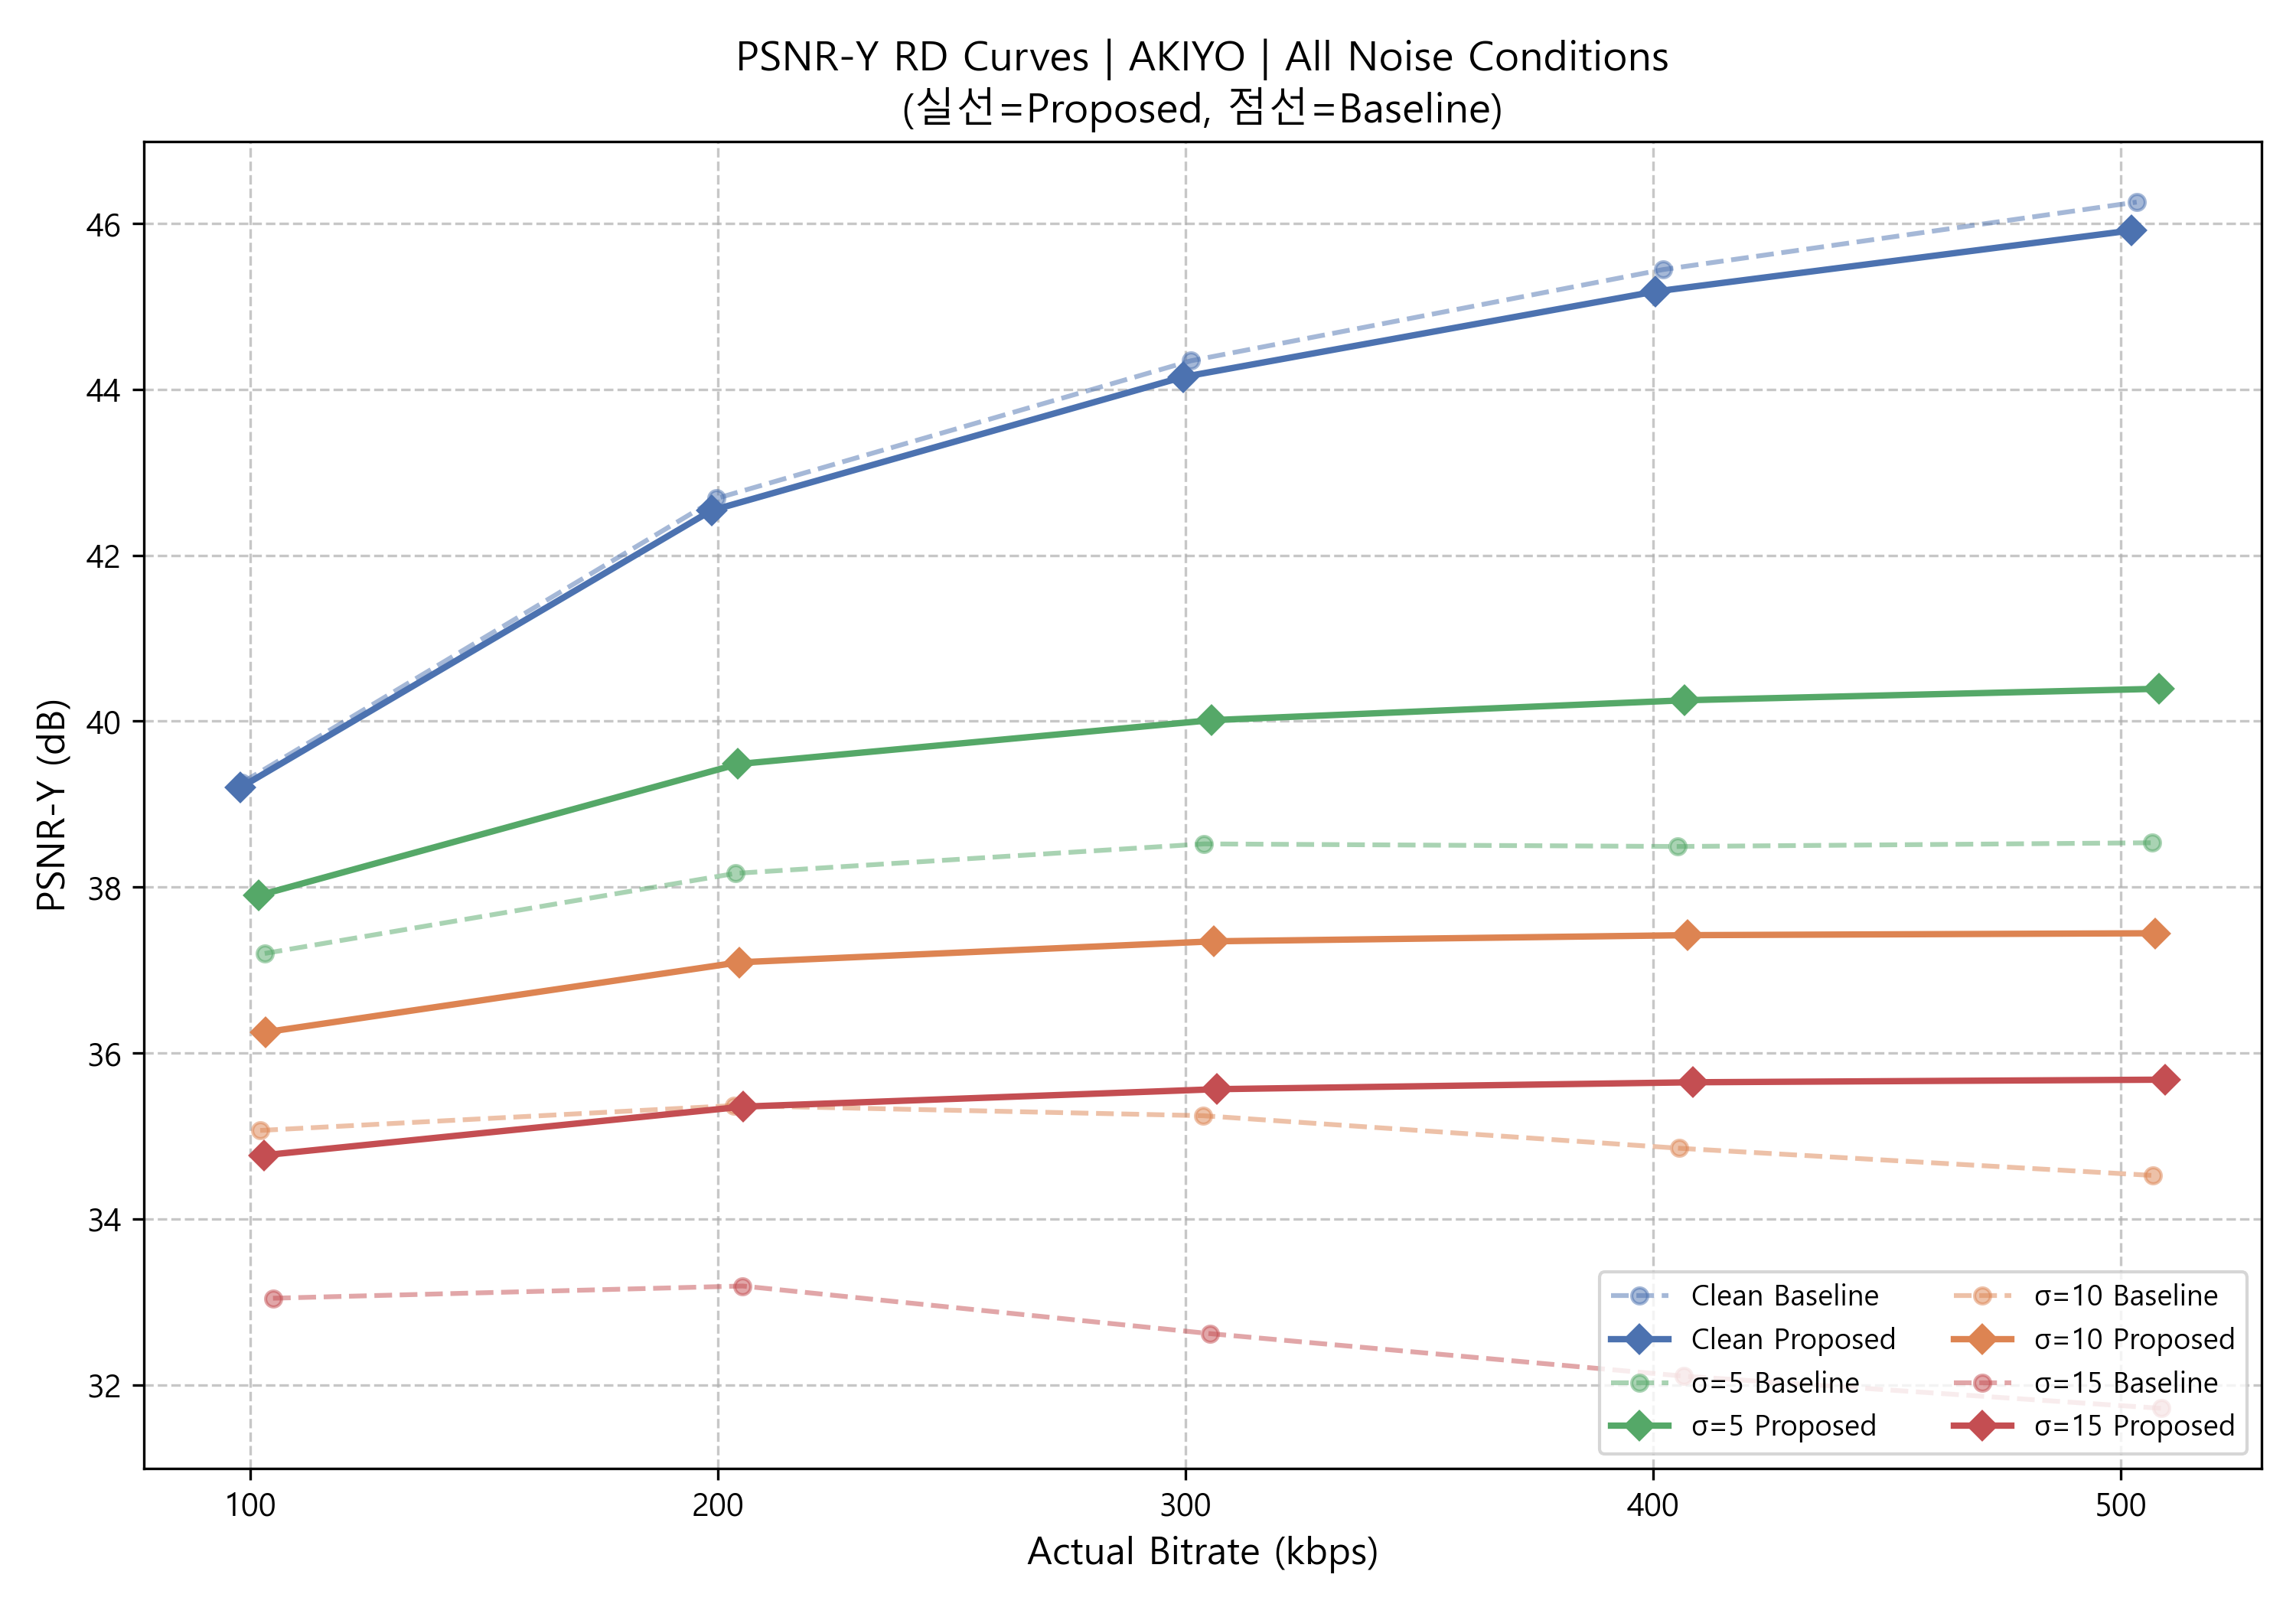
\includegraphics[width=\figwidth]{../outputspaper_full/rd_overlay_psnr_akiyo.png}
\caption{\textit{akiyo} 영상의 잡음 조건별 PSNR RD 곡선}
\label{fig:akiyo_rd}
\end{figure}

\begin{figure}[hbtp]
\centering
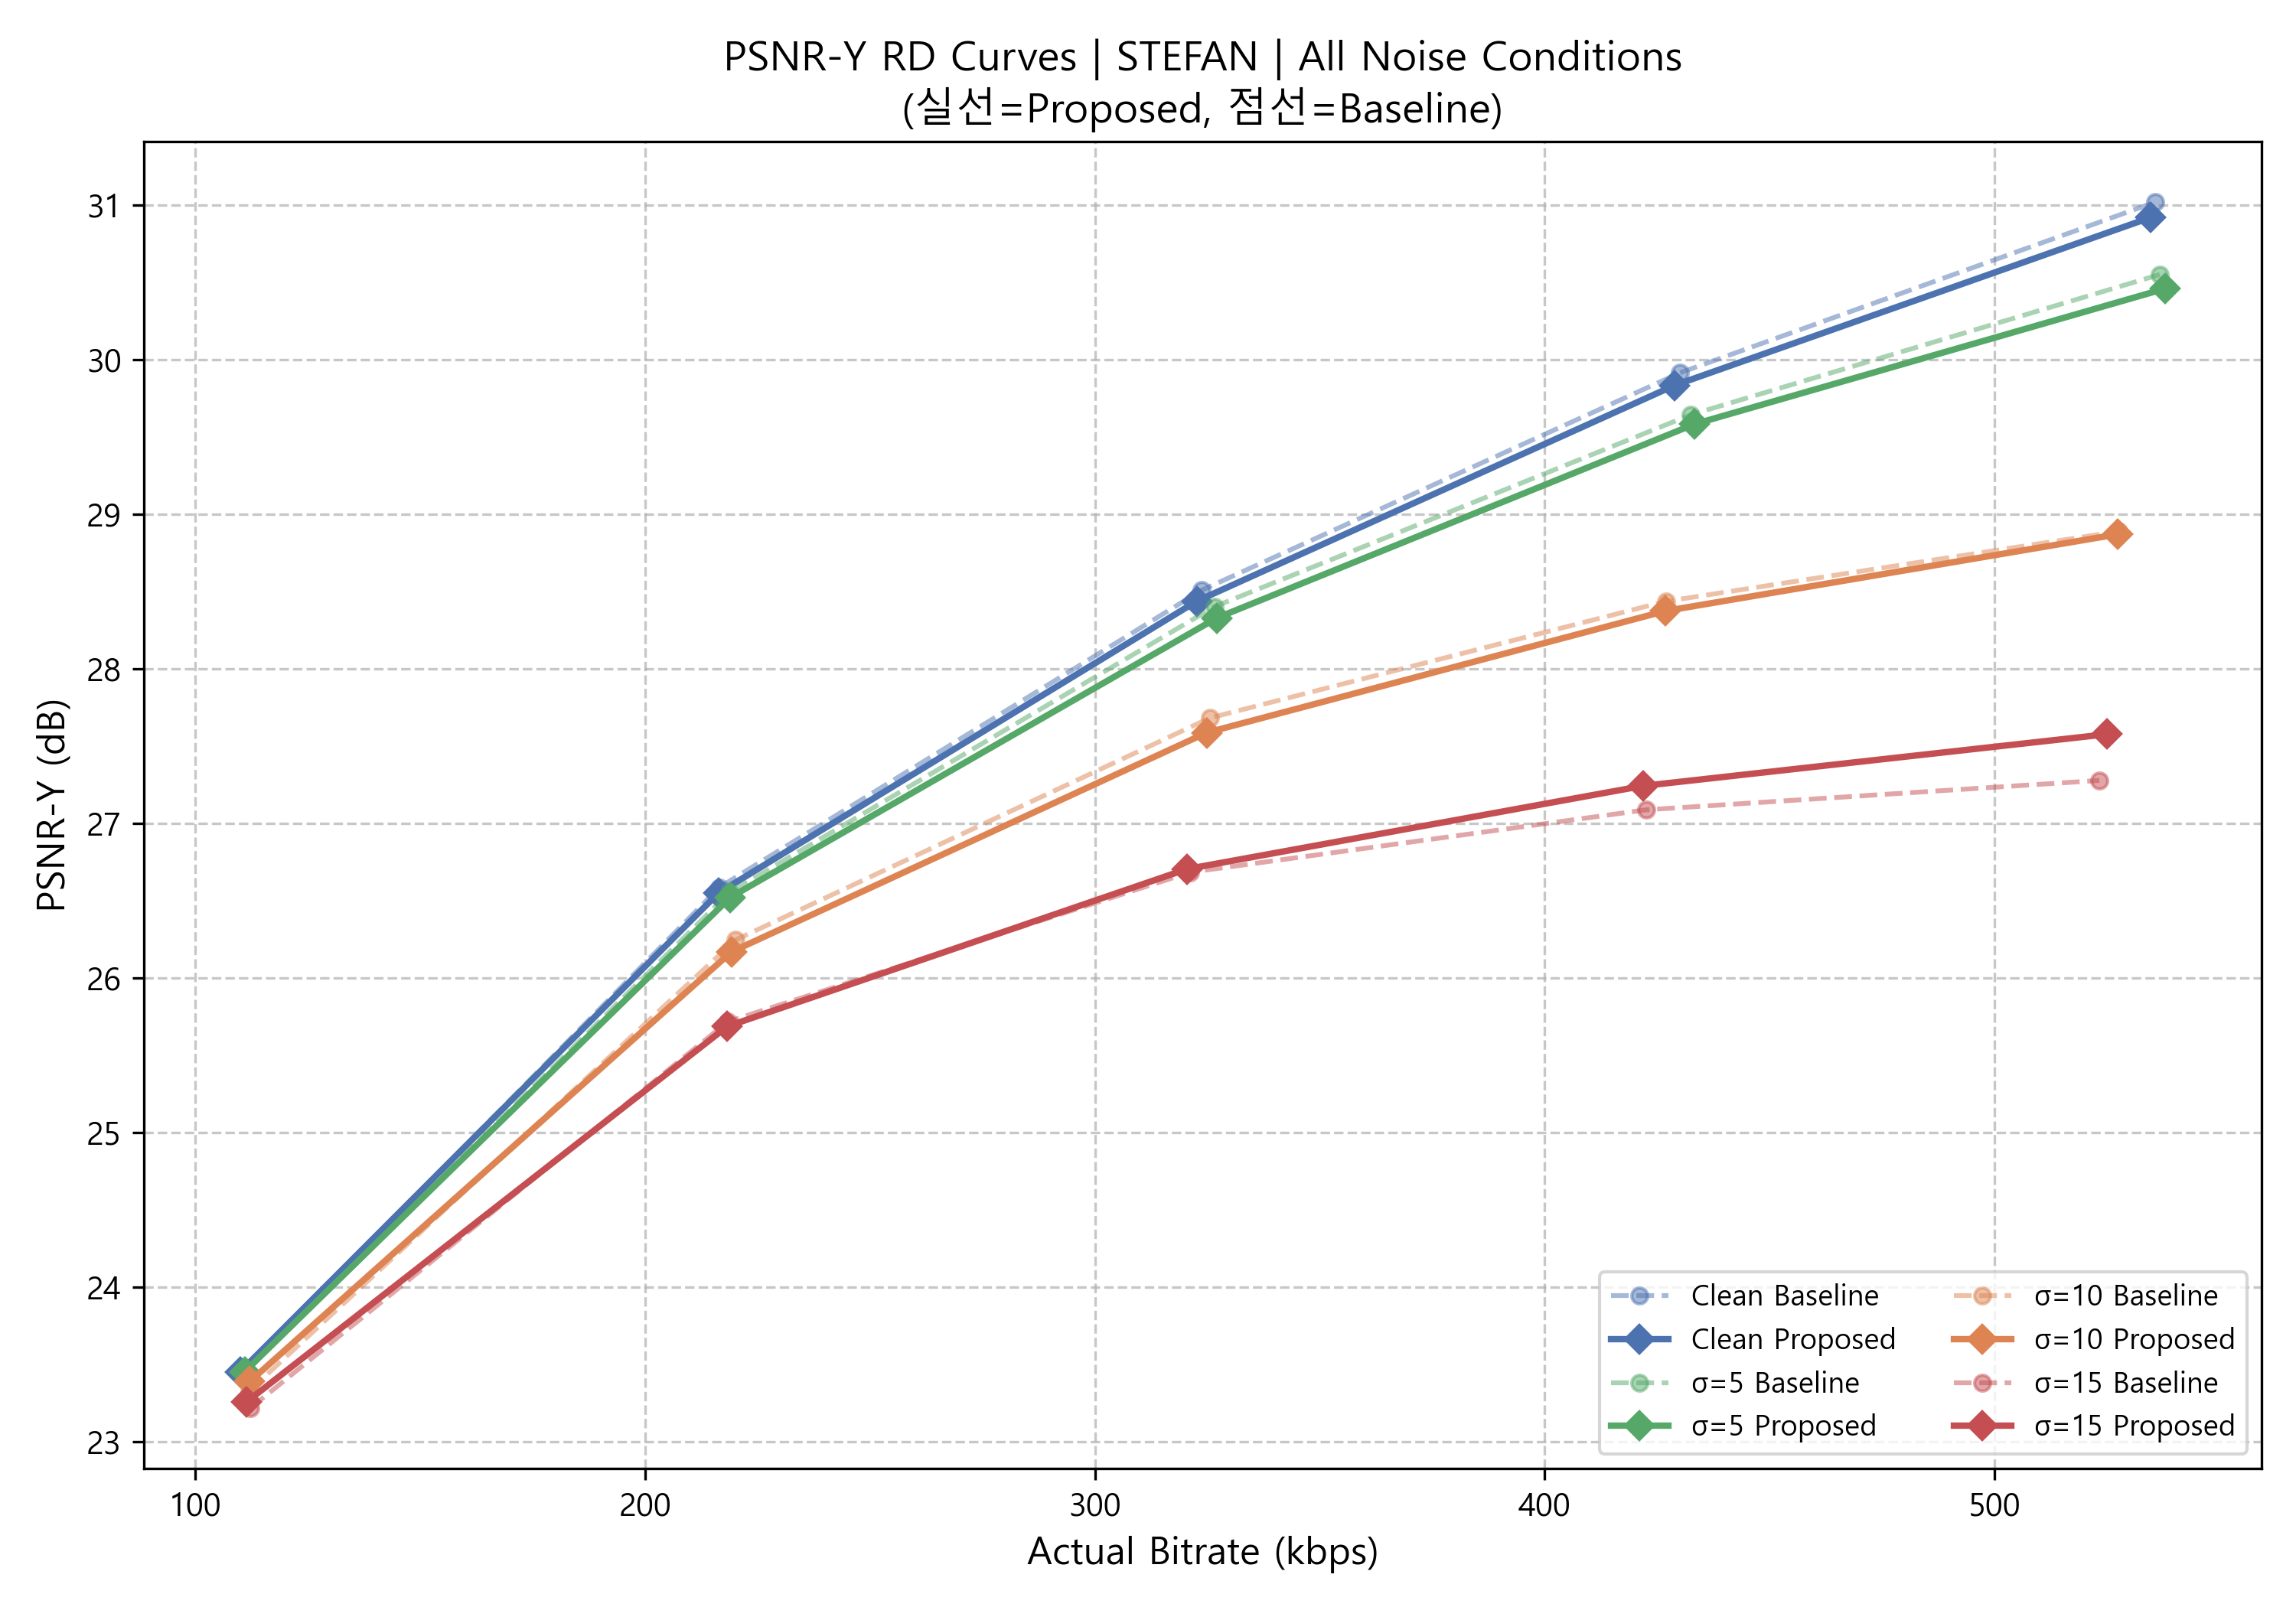
\includegraphics[width=\figwidth]{../outputspaper_full/rd_overlay_psnr_stefan.png}
\caption{\textit{stefan} 영상의 잡음 조건별 PSNR RD 곡선}
\label{fig:stefan_rd}
\end{figure}

\subsection{저비트레이트 구간 분석}
본 연구의 관심은 특히 300 kbps 이하의 저비트레이트 조건이다. 이 구간에서 제안 방법의 이득은 전체 평균과 비슷한 경향을 보였다. \textit{akiyo}는 $\sigma=15$에서 저비트레이트 평균 PSNR 이득이 2.28 dB였으며, \textit{foreman}은 0.59 dB, \textit{mobile}은 0.24 dB였다. 그러나 \textit{stefan}은 같은 조건에서 0.01 dB로 사실상 변화가 없었다.

이 결과는 제안 방법이 저비트레이트에서 잡음 제거 효과를 최종 품질 개선으로 연결할 수 있음을 보여주지만, 그 효과가 영상 내용에 강하게 의존함을 동시에 보여준다. 안정적인 영상에서는 잡음이 비트 예산을 소모하는 주요 요인이므로 전처리 효과가 크다. 반대로 빠른 움직임 영상에서는 제거해야 할 잡음과 보존해야 할 시간축 detail이 더 잘 분리되지 않아 이득이 작아진다.

\begin{figure}[hbtp]
\centering
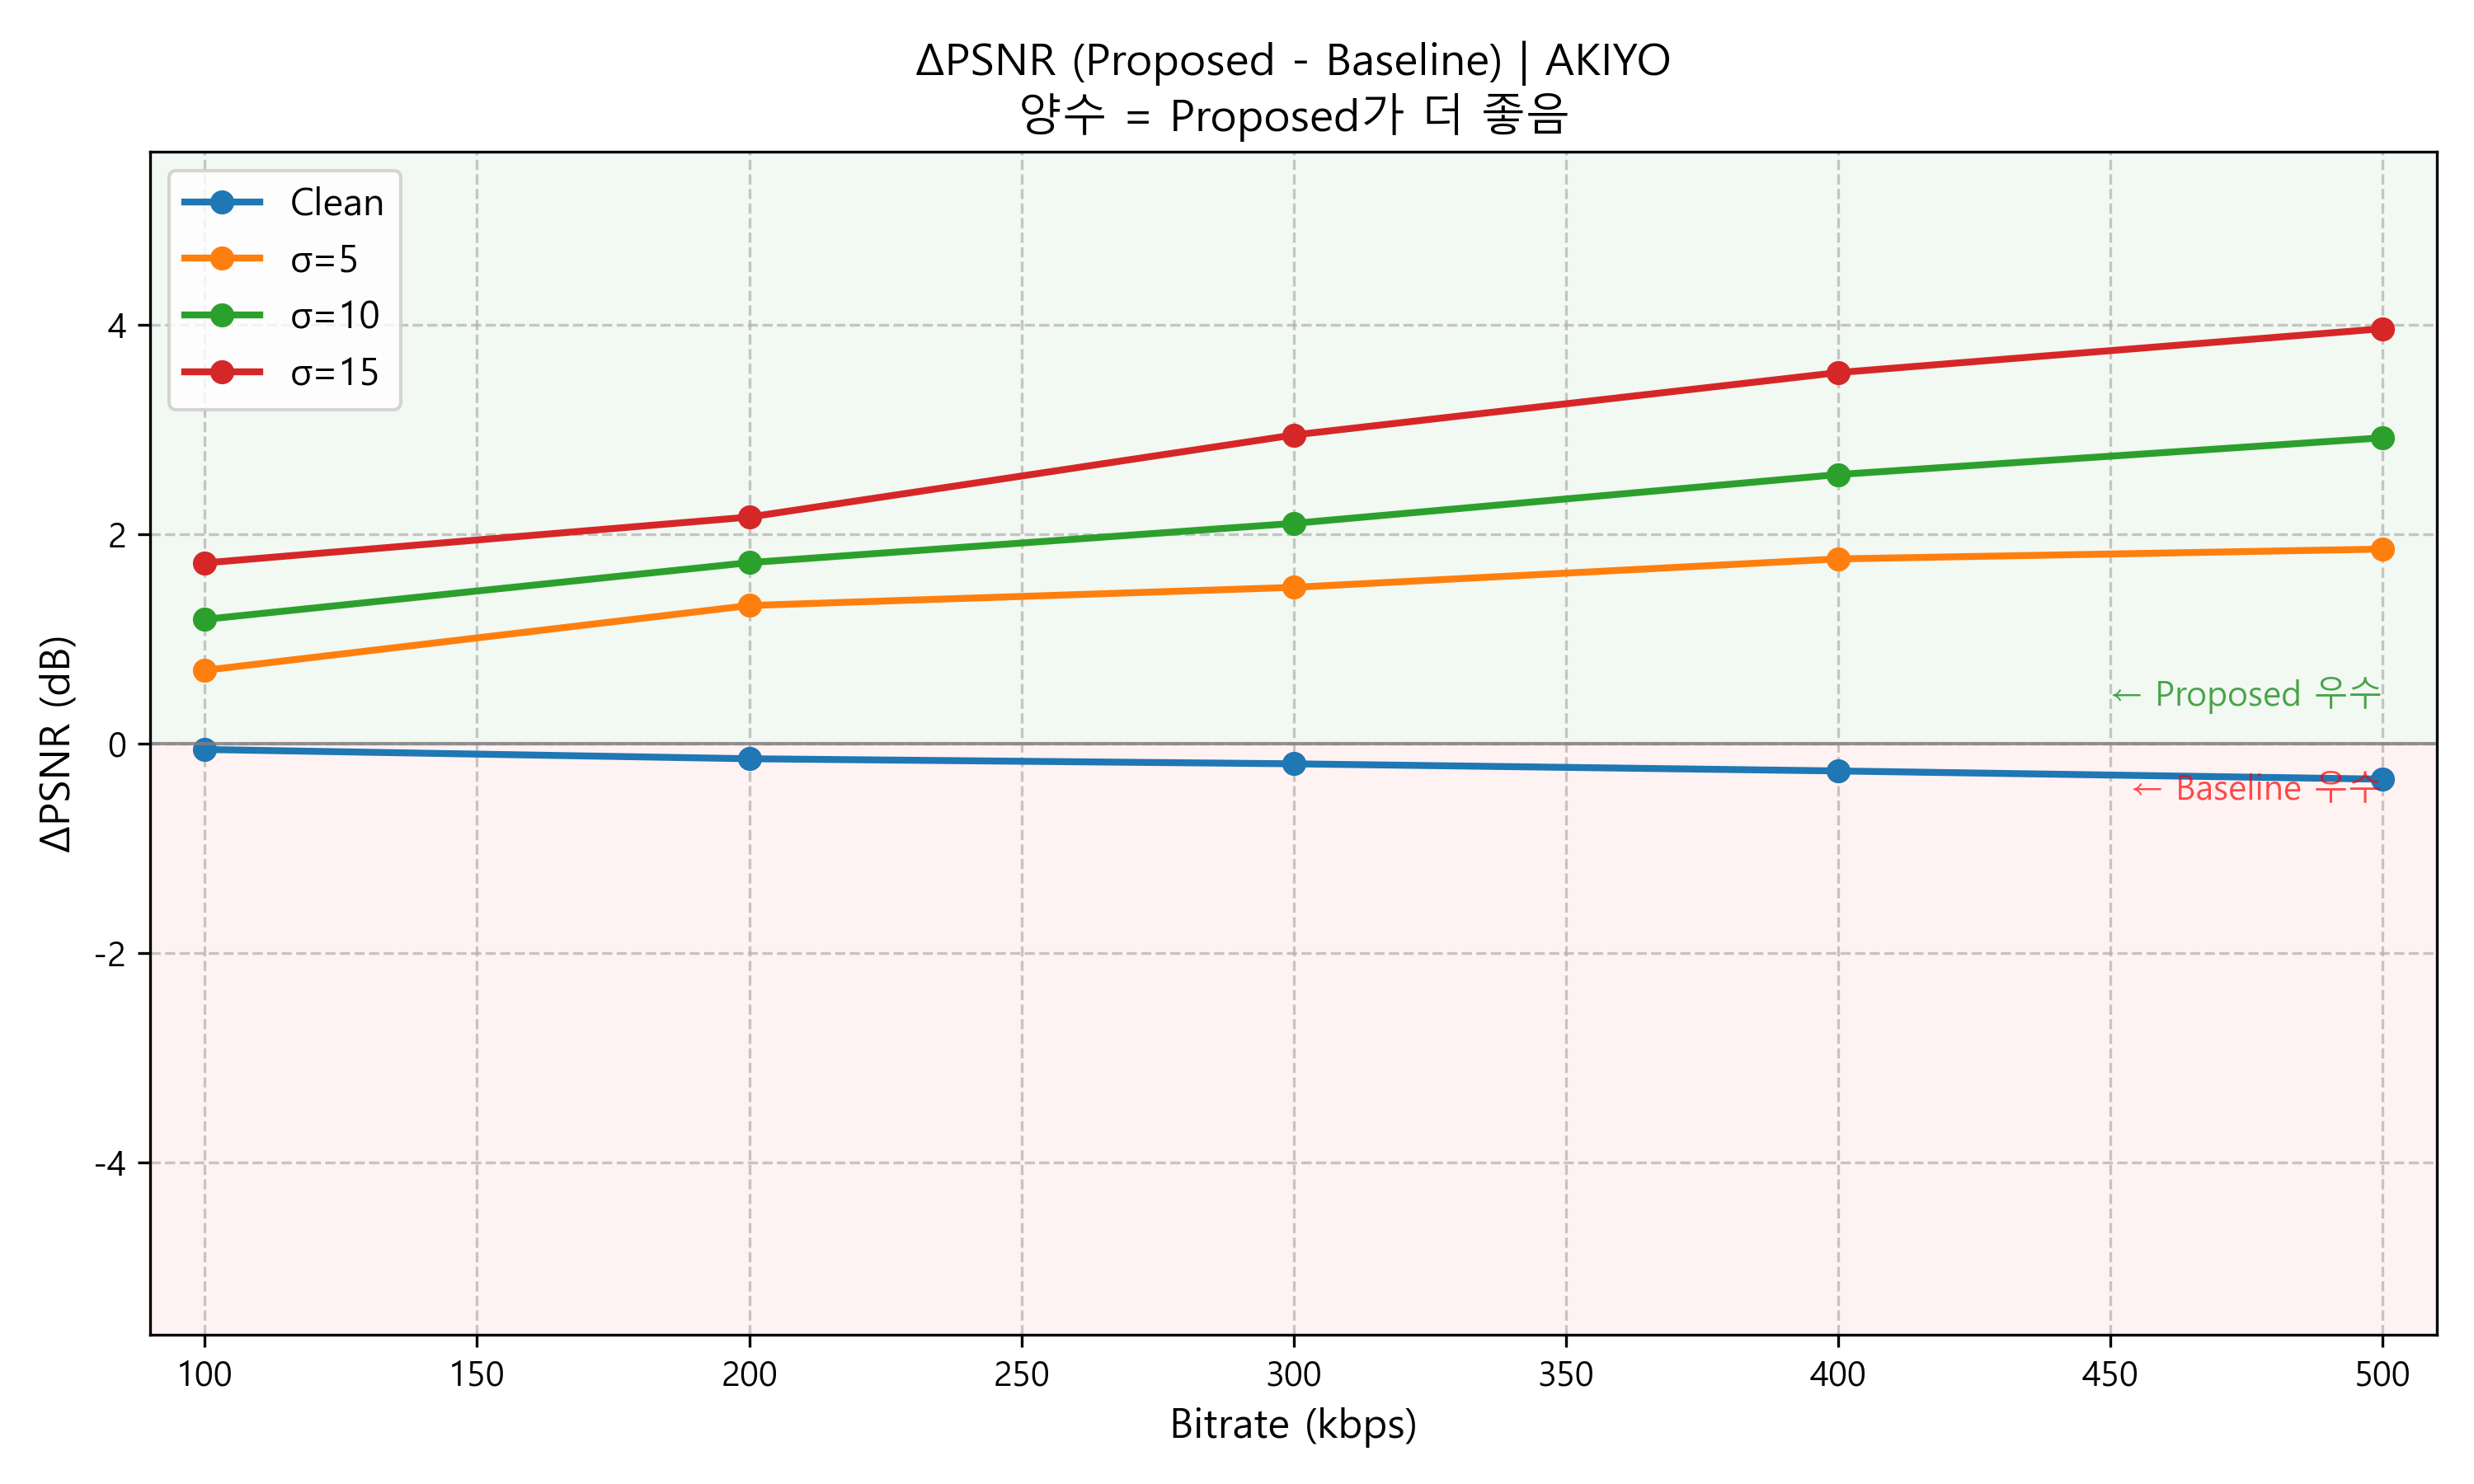
\includegraphics[width=\smallfigwidth]{../outputspaper_full/delta_psnr_akiyo.png}
\caption{\textit{akiyo} 영상에서 bitrate별 $\Delta$PSNR 변화}
\label{fig:delta_akiyo}
\end{figure}

\begin{figure}[hbtp]
\centering
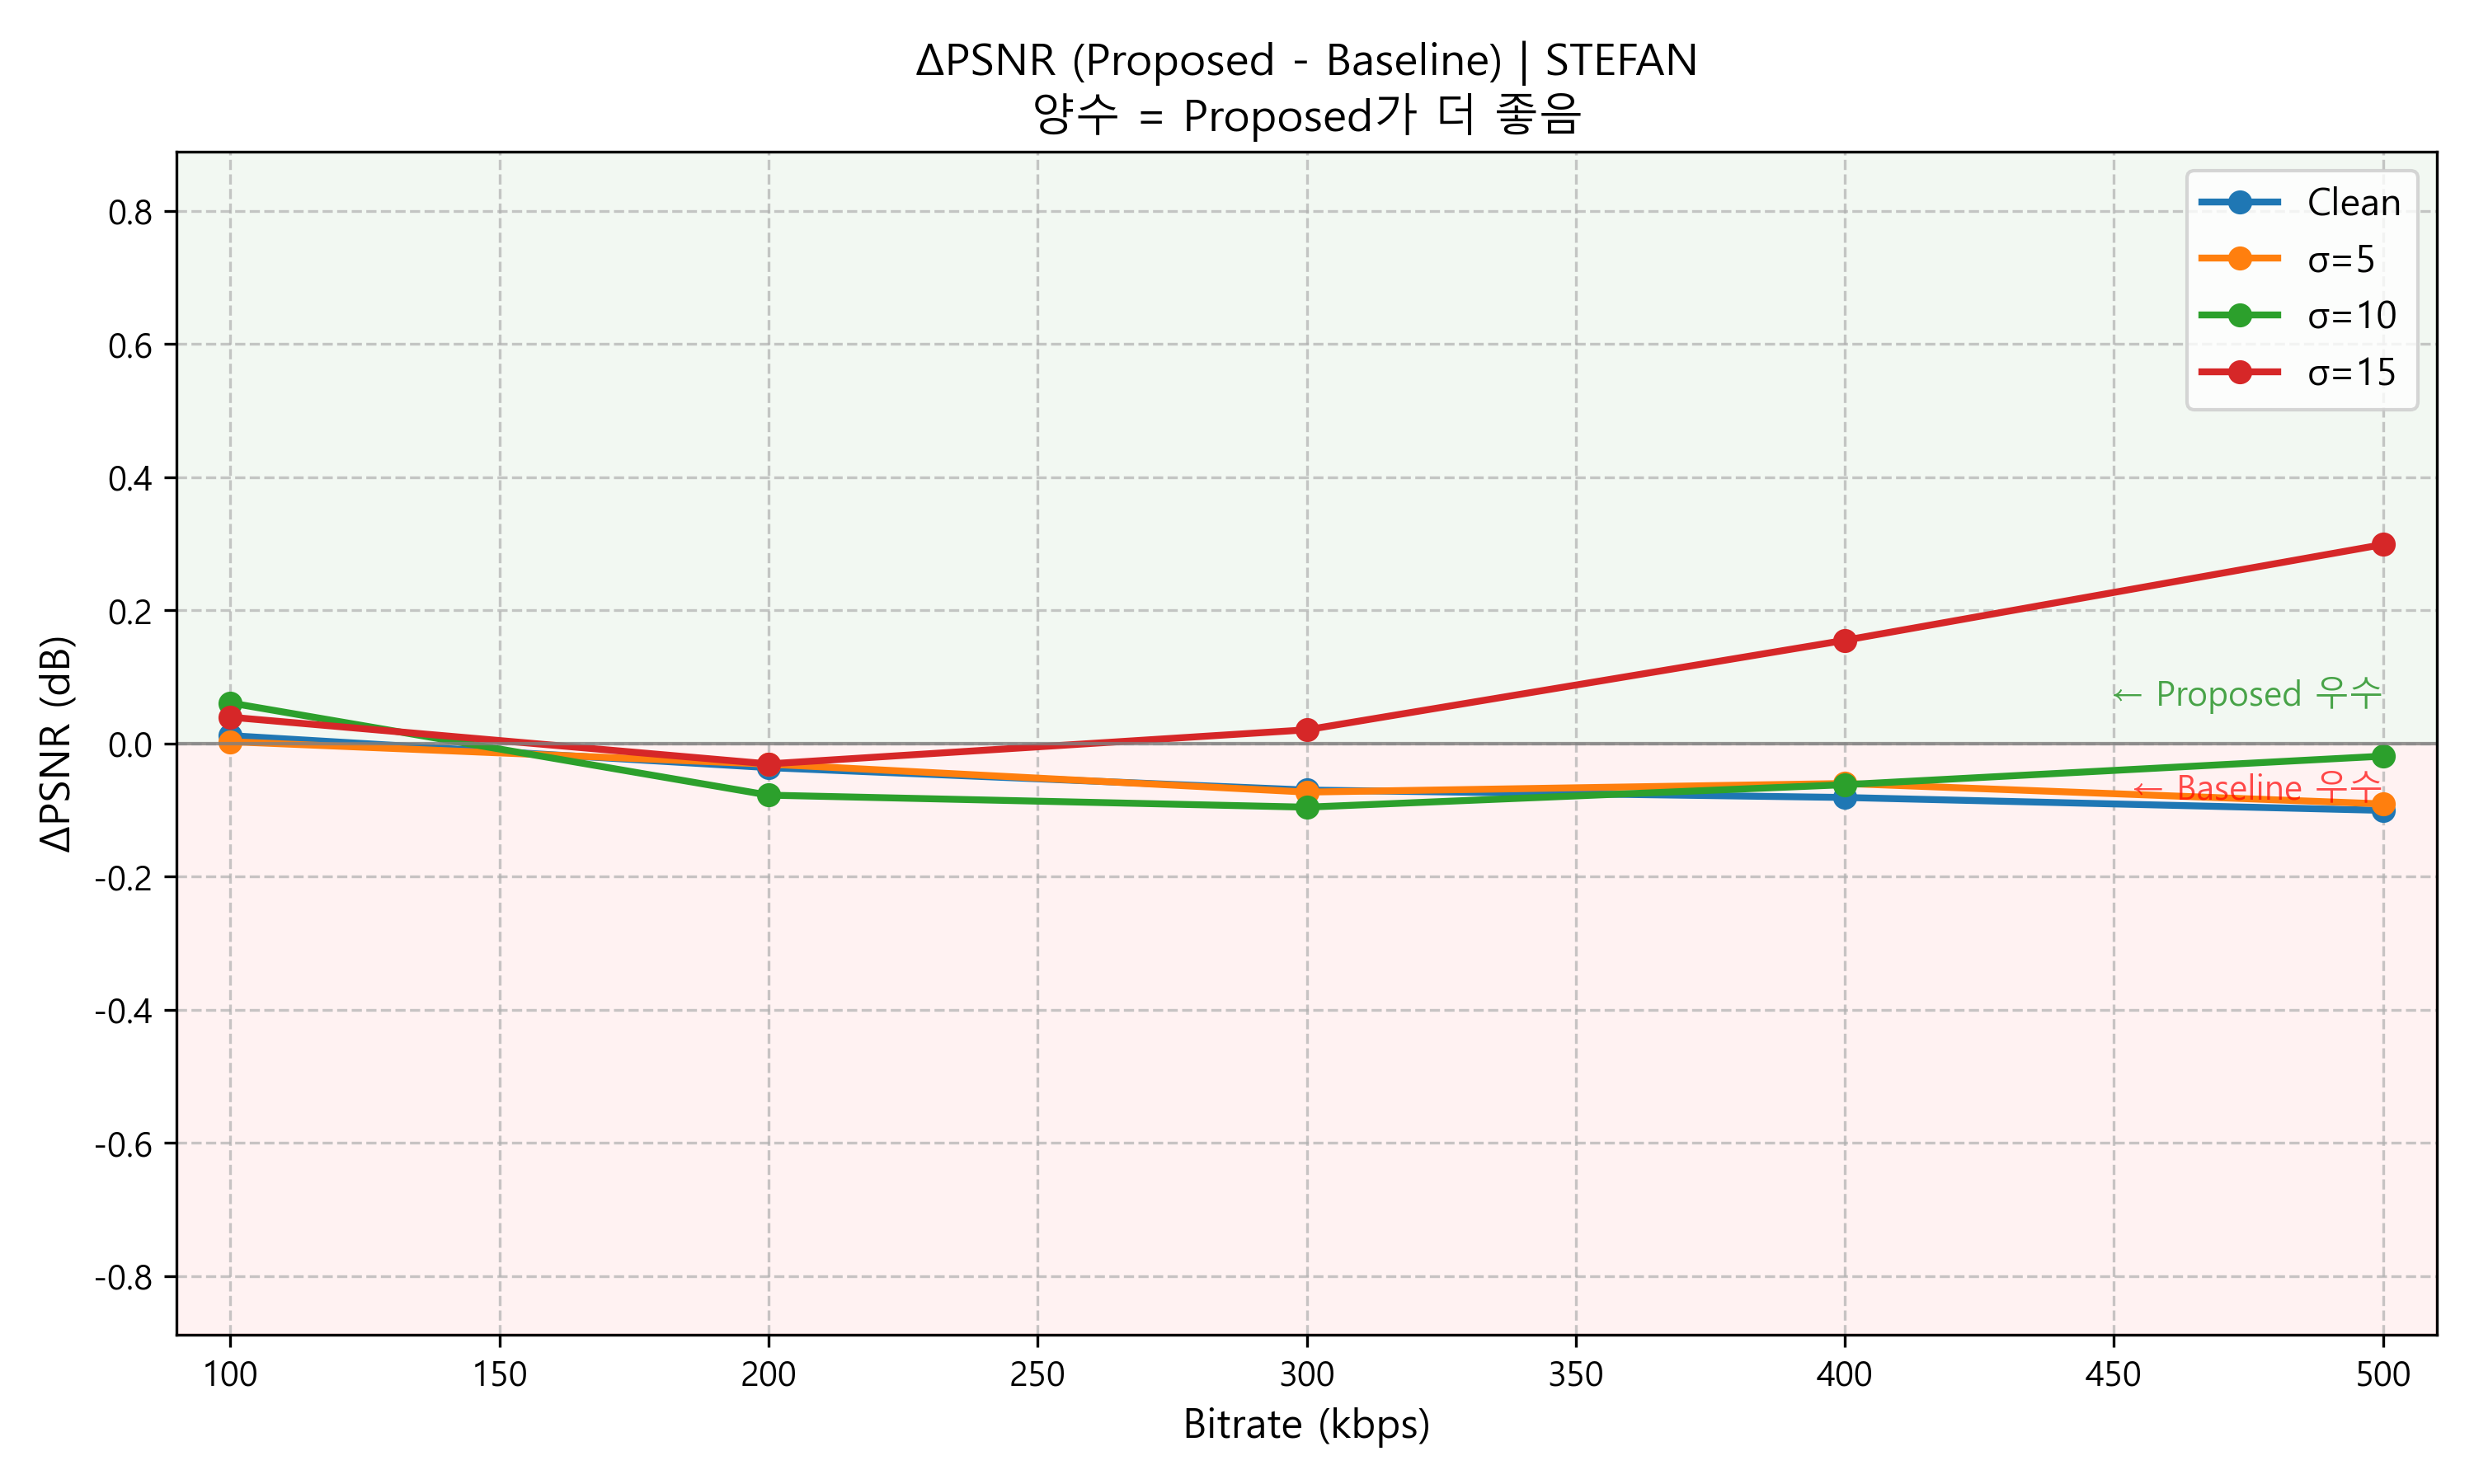
\includegraphics[width=\smallfigwidth]{../outputspaper_full/delta_psnr_stefan.png}
\caption{\textit{stefan} 영상에서 bitrate별 $\Delta$PSNR 변화}
\label{fig:delta_stefan}
\end{figure}

\subsection{비교군과의 관계}
표 \ref{tab:method_sigma15}는 가장 강한 잡음 조건인 $\sigma=15$에서 각 방법의 평균 PSNR 이득을 비교한 것이다. x264 NR과 hqdn3d는 거의 0에 가까운 변화를 보였고, Gaussian blur는 대부분 음수였다. 3D DWT는 \textit{akiyo}, \textit{foreman}, \textit{mobile}, \textit{stefan}에서 모두 양의 이득을 보였으며, 특히 \textit{stefan}에서는 Proposed보다 높은 PSNR을 기록하였다. Proposed는 \textit{akiyo}, \textit{foreman}, \textit{mobile}에서 3D DWT보다 높은 평균 PSNR 이득을 보였으나, 모든 영상에서 항상 최고는 아니었다.

\begin{table}[hbtp]
\centering
\caption{$\sigma=15$ 조건에서 방법별 평균 PSNR 이득(dB)}
\label{tab:method_sigma15}
\begin{tabular}{lrrrrr}
\toprule
영상 & x264 NR & hqdn3d & 3D DWT & Gaussian & Proposed \\
\midrule
\textit{akiyo} & 0.00 & 0.01 & 1.64 & -0.56 & 2.87 \\
\textit{foreman} & 0.00 & 0.00 & 0.79 & -1.53 & 0.94 \\
\textit{mobile} & 0.00 & 0.00 & 0.19 & -3.80 & 0.36 \\
\textit{stefan} & 0.00 & 0.00 & 0.35 & -2.94 & 0.10 \\
\bottomrule
\end{tabular}
\end{table}

이 비교는 본 연구의 결론을 더 구체적으로 만든다. Proposed는 단순 공간 blur나 hqdn3d보다 noisy low-bitrate 조건에서 더 강한 경우가 많고, 3D DWT보다도 저움직임 및 중간 움직임 영상에서 우수했다. 그러나 고속 움직임 영상에서는 3D DWT가 더 보수적인 smoothing을 수행하여 PSNR 기준으로 더 나은 결과를 낼 수 있다. 따라서 DT-CWT의 방향성은 장점이지만, 움직임이 매우 복잡한 경우에는 thresholding 강도와 시간축 처리 방식이 더 정교해야 한다.

\subsection{블로킹, 구조 유사도, 시간 품질 지표 분석}
표 \ref{tab:aux_gain}은 $\sigma=15$ 조건에서 PSNR-B, MS-SSIM, GBIM, STRRED-like score의 raw delta를 정리한 것이다. 표의 값은 모두 \textit{Proposed - Baseline}으로 계산하였으므로, PSNR-B와 MS-SSIM은 양수일수록 좋고, GBIM과 STRRED-like score는 음수일수록 좋다. 이 방식은 그래프와 표의 부호를 원자료 계산식과 일치시켜, 어떤 지표에서 실제 값이 증가했는지 또는 감소했는지를 직접 확인할 수 있게 한다.

PSNR-B는 네 영상 모두에서 양수였고, 특히 \textit{akiyo}와 \textit{foreman}에서 각각 3.87 dB, 1.78 dB 증가하였다. 이는 제안 방법이 단순히 픽셀 오차를 줄이는 것에 그치지 않고, 저비트레이트 x264 이후의 블록 경계 왜곡도 줄이는 데 기여했음을 의미한다. MS-SSIM 또한 모든 noisy 조건에서 양수였으며, $\sigma=15$에서는 네 영상 모두 구조 유사도가 개선되었다. 따라서 PSNR-B와 MS-SSIM을 중심 지표로 사용하는 것은 본 연구의 목적과 잘 맞는다.

GBIM은 모든 noisy 조건에서 raw delta가 음수였다. 특히 $\sigma=15$에서는 \textit{akiyo}, \textit{foreman}, \textit{mobile}, \textit{stefan}의 GBIM delta가 각각 -2.22, -2.03, -1.38, -1.67로 감소했으므로, 제안 방법이 블록 경계의 불연속을 완화하는 경향이 있음을 확인할 수 있다. 다만 GBIM은 경계 불연속 자체를 보는 지표이므로, 지나친 smoothing이 있을 때도 좋아질 수 있다. 따라서 GBIM은 PSNR-B와 함께 해석할 때 가장 의미가 있다.

반면 STRRED-like score는 영상별로 엇갈렸다. \textit{akiyo}에서는 $\sigma=15$에서 -0.90으로 감소했지만, \textit{foreman}, \textit{mobile}, \textit{stefan}에서는 각각 0.71, 0.28, 0.21로 증가하였다. 이는 DT-CWT 전처리가 저움직임 영상의 시공간 통계는 clean 원본에 가깝게 만들지만, 움직임이나 질감이 복잡한 영상에서는 시간적 bandpass 통계를 오히려 바꿀 수 있음을 의미한다. 그러므로 STRRED-like score는 제안 방법의 한계를 보여주는 중요한 보조 지표로 해석된다.

\begin{table}[hbtp]
\centering
\caption{$\sigma=15$ 조건에서 제안 방법의 raw metric delta(Proposed - Baseline)}
\label{tab:aux_gain}
\begin{tabular}{lrrrr}
\toprule
영상 & PSNR-B(dB) & MS-SSIM & GBIM & STRRED-like \\
\midrule
\textit{akiyo} & 3.87 & 0.0363 & -2.22 & -0.90 \\
\textit{foreman} & 1.78 & 0.0208 & -2.03 & 0.71 \\
\textit{mobile} & 0.26 & 0.0070 & -1.38 & 0.28 \\
\textit{stefan} & 0.21 & 0.0049 & -1.67 & 0.21 \\
\bottomrule
\end{tabular}
\end{table}

따라서 제안 방법의 효과는 ``화질 지표 전체가 항상 동시에 좋아진다''로 해석하면 안 된다. PSNR-B와 MS-SSIM의 양의 delta, GBIM의 음의 delta는 noisy 조건에서 제안 방법의 장점을 지지하지만, STRRED-like score의 양의 delta는 움직임이 있는 영상에서 시간적 통계 변화라는 한계를 드러낸다. 이 때문에 본 연구의 결론은 ``DT-CWT 전처리가 항상 우수하다''가 아니라, ``잡음과 블로킹 완화에는 효과적이지만 시간적 구조 보존을 위해 조건부 적용과 강도 조절이 필요하다''가 되어야 한다.

\subsection{BD-Rate 결과와 해석상의 주의}
BD-Rate는 RD 곡선을 하나의 수치로 요약할 수 있다는 장점이 있지만, 본 실험의 모든 지표에 안정적으로 적용되지는 않았다. PSNR 기준 BD-Rate는 \textit{foreman}, \textit{mobile}, \textit{stefan}의 높은 잡음 조건에서 음수로 나타나 제안 방법의 압축 효율 개선을 지지한다. \textit{akiyo}의 $\sigma=5$에서도 PSNR 기준 BD-Rate는 -45.84\%로 계산되었다.

다만 \textit{akiyo}의 $\sigma=10,15$처럼 제안 방법과 baseline의 RD 곡선 품질 구간이 충분히 겹치지 않는 조건에서는 BD-Rate가 정의되지 않았다. 또한 MS-SSIM은 값의 범위가 0과 1 사이로 좁고, 실험 결과가 1에 가까운 구간에 몰리며, 일부 RD 곡선이 완전히 단조 증가하지 않았다. 이 경우 다항식 기반 BD-Rate 계산이 매우 불안정해져 비현실적으로 큰 값이 나올 수 있다. 따라서 본 연구에서는 MS-SSIM BD-Rate를 결론 지표로 사용하지 않고, 그림 \ref{fig:metric_deltas}와 같이 raw metric delta와 win-rate를 중심으로 해석하였다.

\begin{figure}[hbtp]
\centering
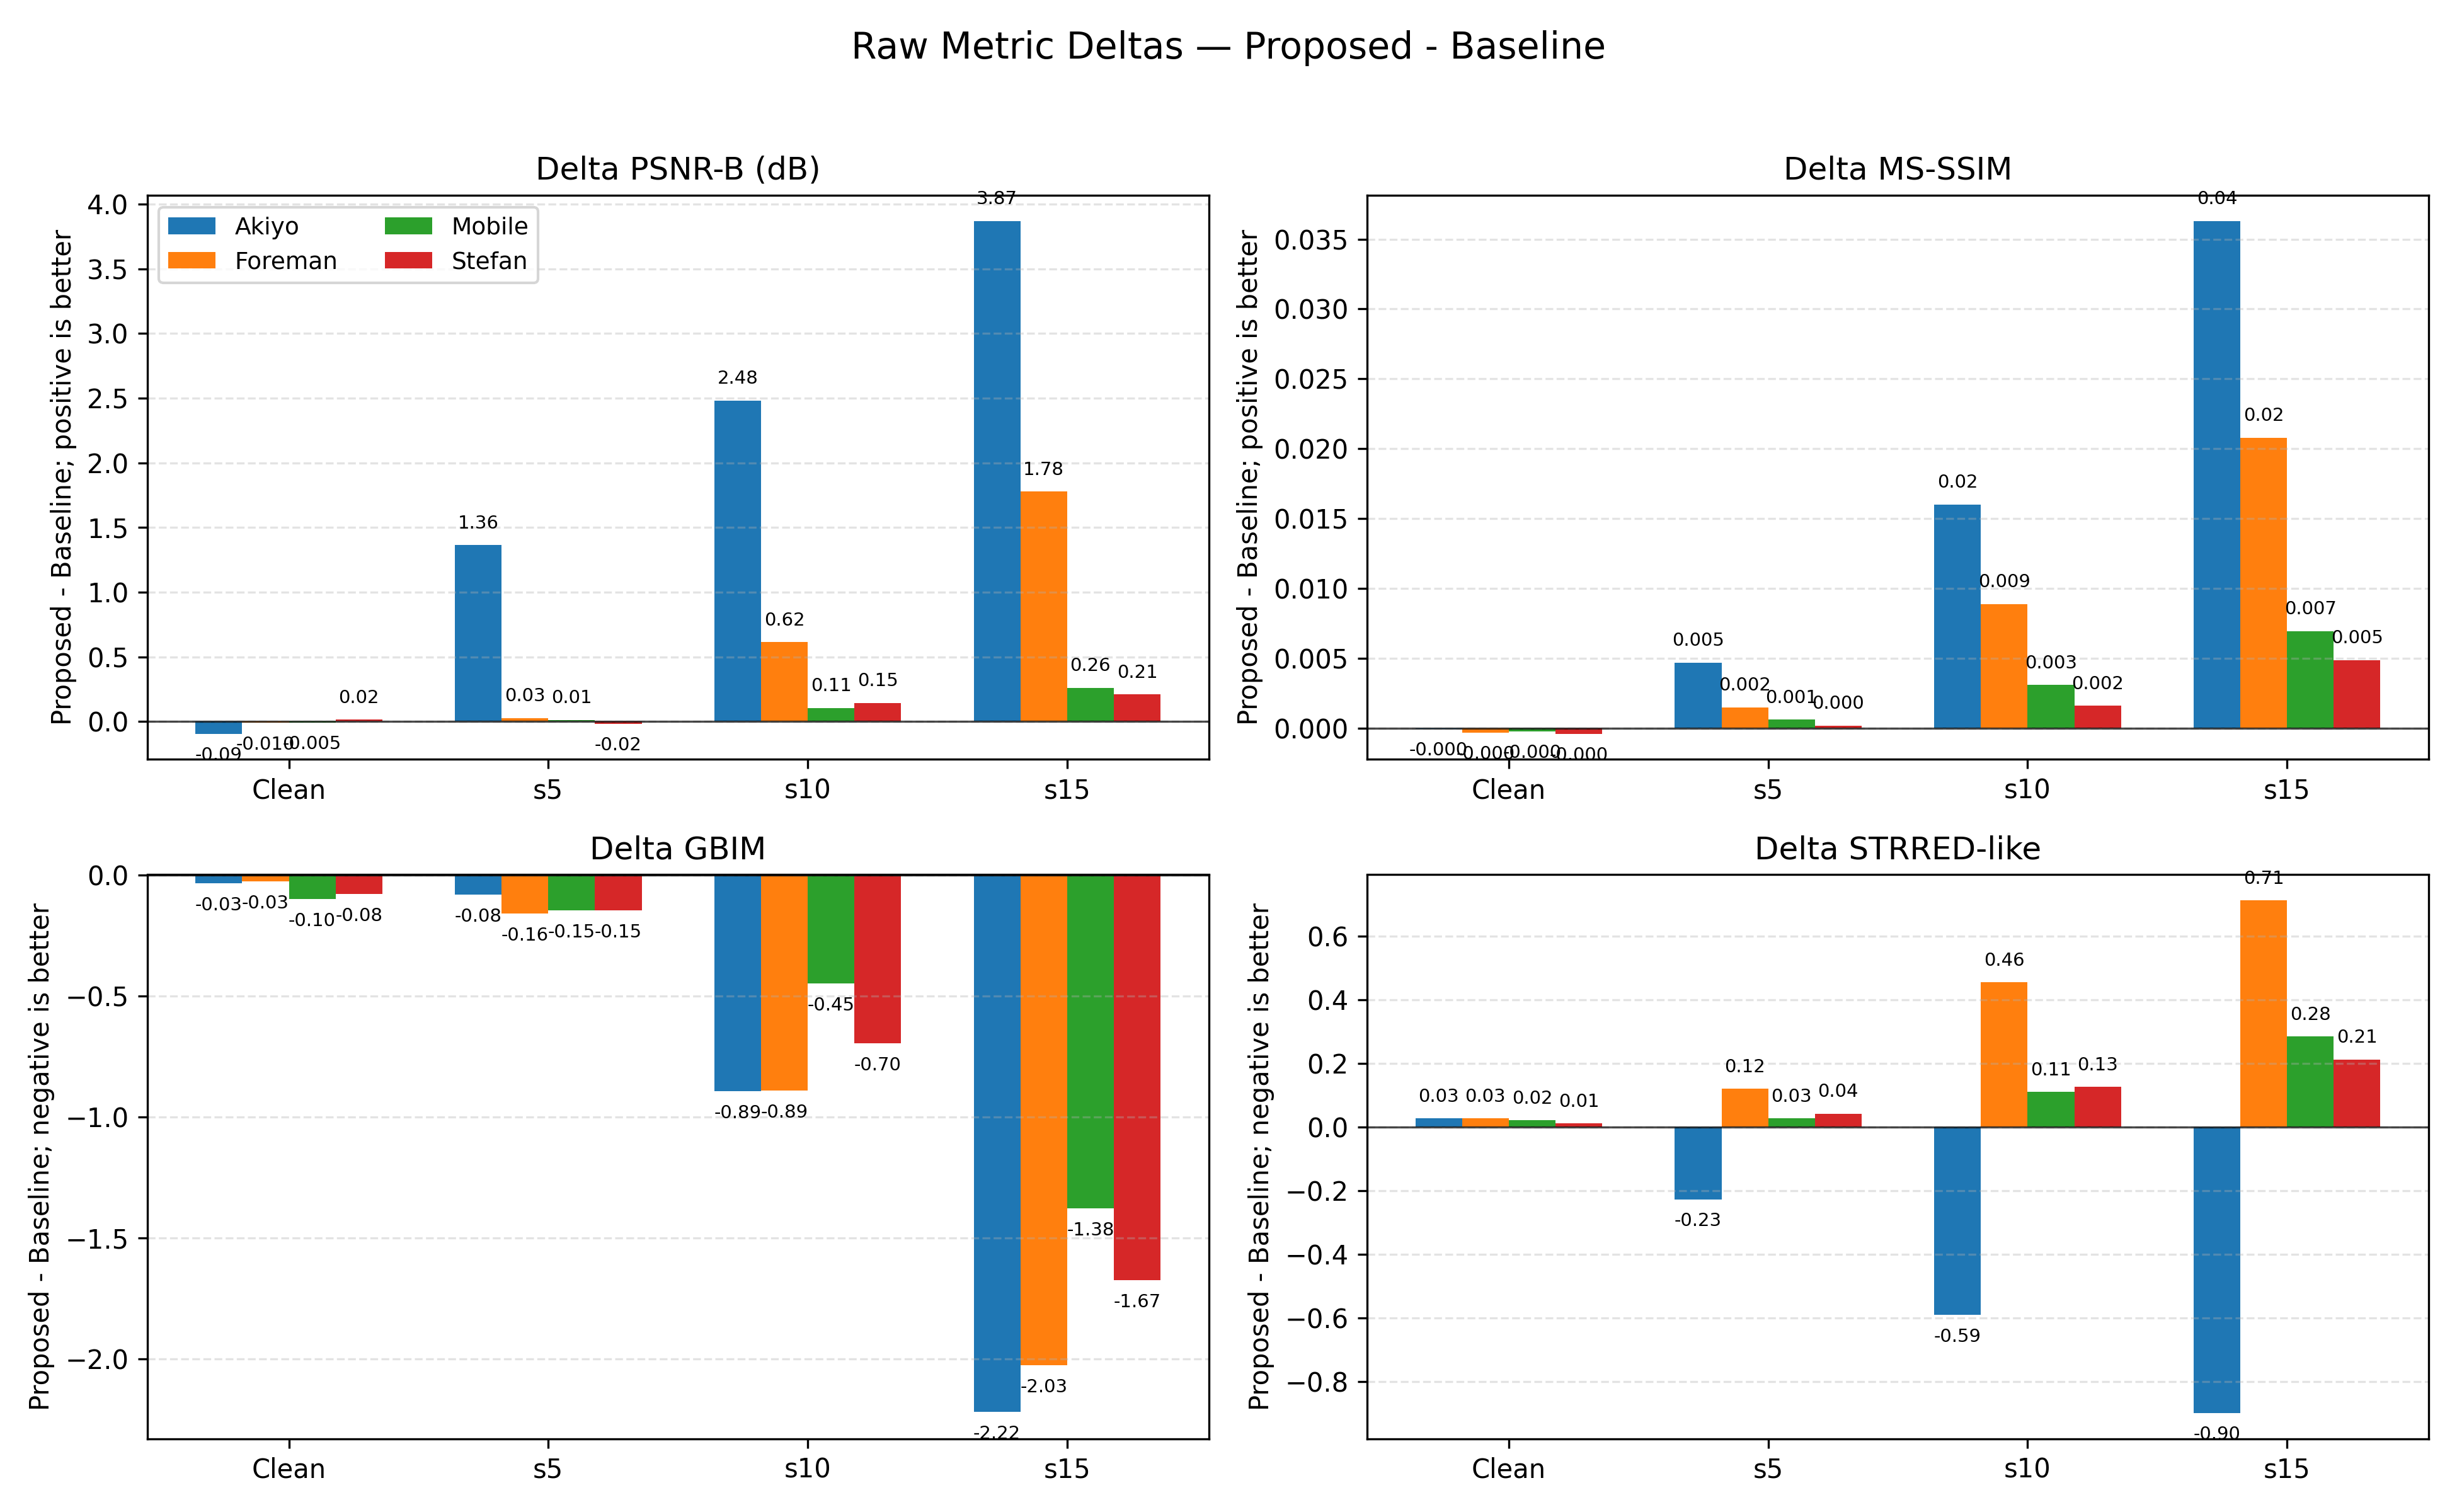
\includegraphics[width=\figwidth]{../outputspaper_full/cross_condition_metric_deltas.png}
\caption{영상 및 잡음 조건별 raw metric delta 비교. 모든 값은 Proposed - Baseline이며, PSNR-B와 MS-SSIM은 양수가 좋고 GBIM과 STRRED-like score는 음수가 좋다.}
\label{fig:metric_deltas}
\end{figure}

\subsection{Pre/Post 비교와 codec gain}
전처리-only 결과와 post-x264 결과를 비교하면, 3D DT-CWT가 입력 noisy 영상을 clean 원본에 더 가깝게 만드는 효과는 분명하다. 그러나 그 이득이 인코딩 이후 모두 유지되지는 않았다. 표 \ref{tab:codec_gain}은 $\sigma=15$에서 PSNR 기준 pre/post 이득과 codec gain을 비교한 것이다. 모든 영상에서 $\Delta_{\mathrm{pre}}$가 $\Delta_{\mathrm{post}}$보다 컸고, codec gain은 음수였다.

\begin{table}[hbtp]
\centering
\caption{$\sigma=15$ 조건에서 PSNR 기준 pre/post 이득과 codec gain}
\label{tab:codec_gain}
\begin{tabular}{lrrr}
\toprule
영상 & $\Delta_{\mathrm{pre}}$ & $\Delta_{\mathrm{post}}$ & codec gain \\
\midrule
\textit{akiyo} & 8.56 & 2.87 & -5.69 \\
\textit{foreman} & 5.51 & 0.94 & -4.57 \\
\textit{mobile} & 3.24 & 0.36 & -2.88 \\
\textit{stefan} & 3.05 & 0.10 & -2.95 \\
\bottomrule
\end{tabular}
\end{table}

이 결과는 연구 가설 중 ``x264가 전처리 이득을 증폭할 수 있다''는 강한 형태를 지지하지 않는다. 오히려 현재 결과는 \textbf{전처리로 얻은 이득의 일부가 x264 이후에도 남아 최종 품질 개선으로 이어진다}는 보수적인 해석을 지지한다. 즉 제안 방법의 핵심 가치는 codec-aware amplification이 아니라, noisy low-bitrate 조건에서 불필요한 잡음 성분을 줄여 최종 압축 결과의 손실을 완화하는 데 있다.

\begin{figure}[hbtp]
\centering
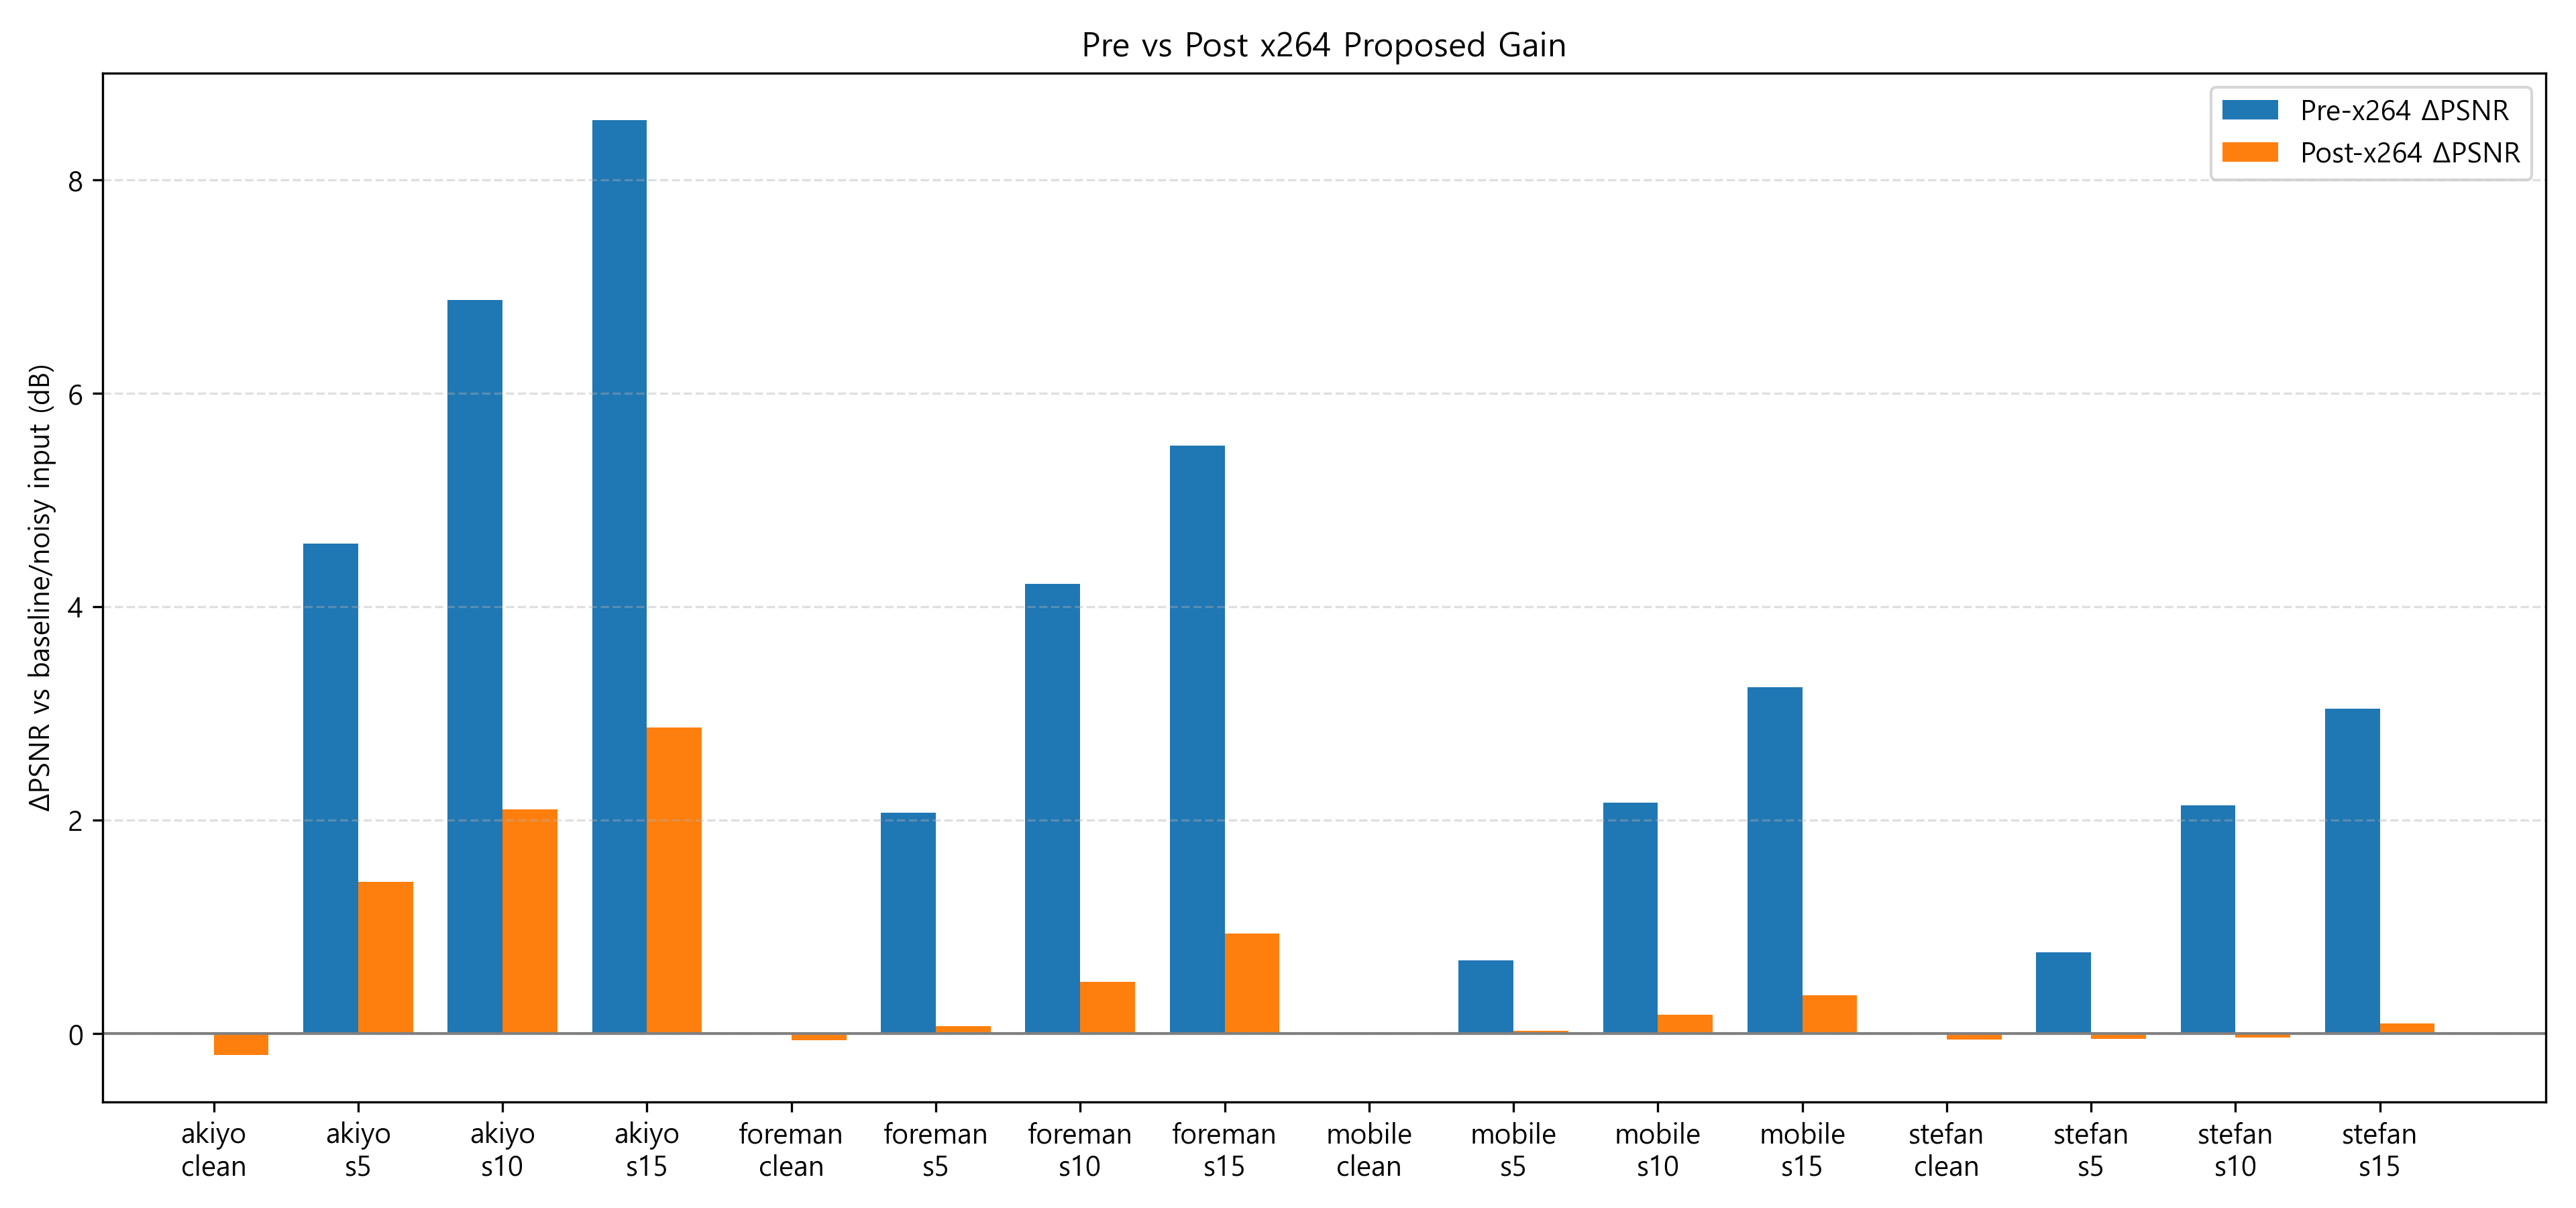
\includegraphics[width=\smallfigwidth]{../outputspaper_full/pre_post_delta_psnr.png}
\caption{제안 방법의 pre-x264 및 post-x264 PSNR 이득 비교}
\label{fig:prepost}
\end{figure}

\begin{figure}[hbtp]
\centering
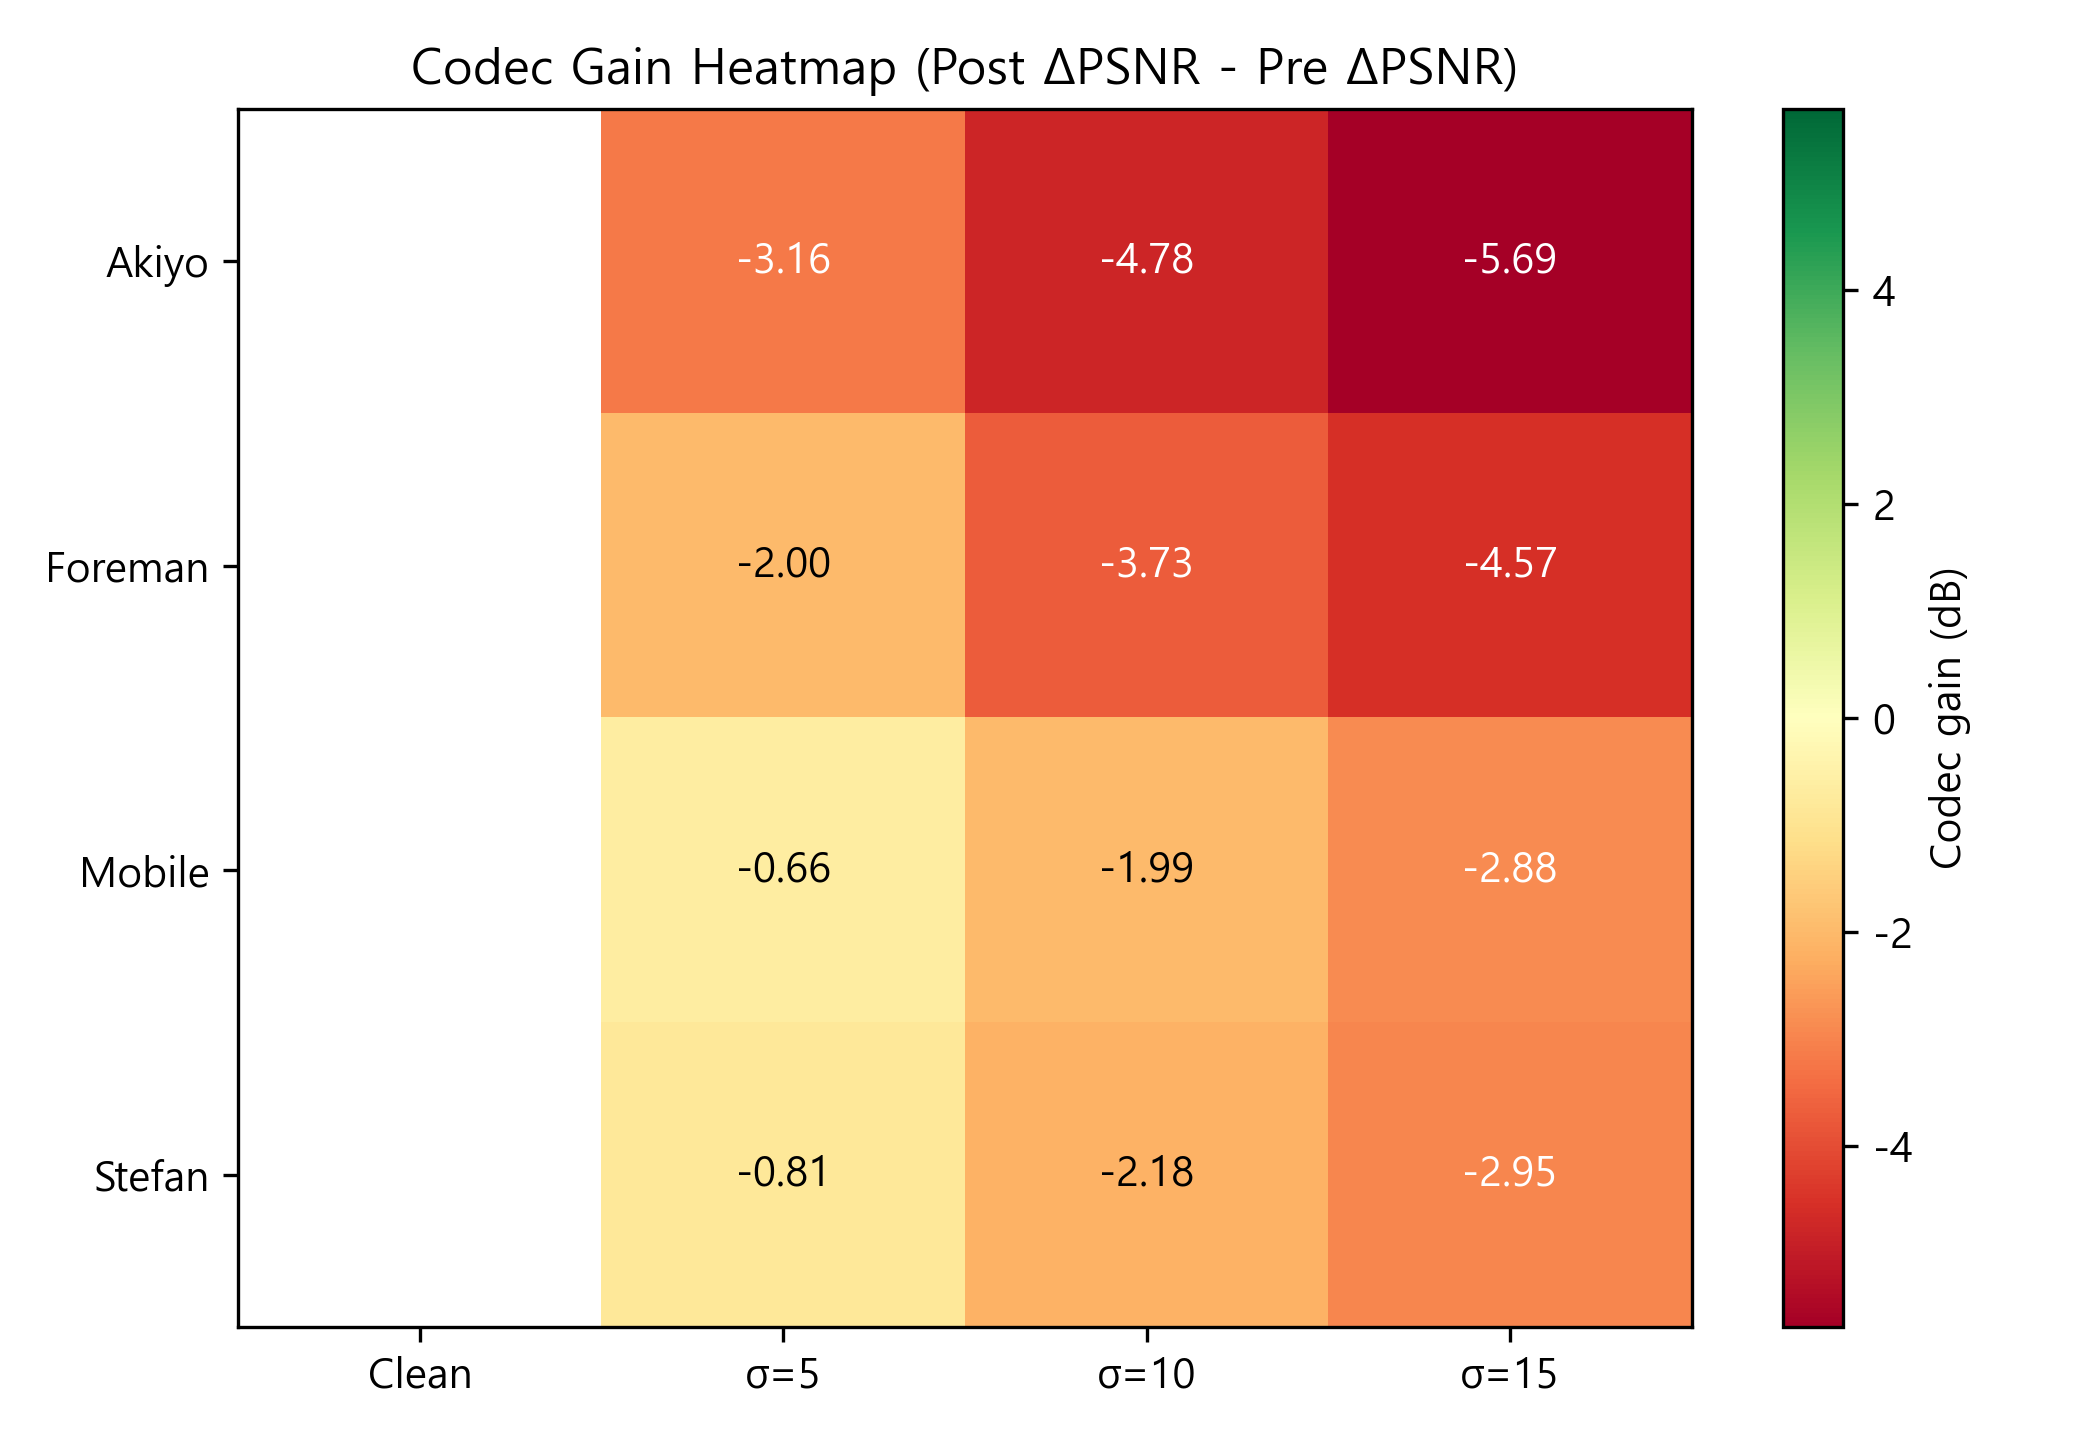
\includegraphics[width=\smallfigwidth]{../outputspaper_full/codec_gain_heatmap.png}
\caption{조건별 codec gain heatmap}
\label{fig:codec_gain}
\end{figure}

\subsection{종합 논의}
실험 결과는 네 가지 결론으로 정리된다. 첫째, 3D DT-CWT 전처리는 clean 입력에는 불리하거나 거의 이득이 없다. 이는 전처리가 잡음과 실제 고주파 구조를 완벽하게 구분하지 못하기 때문이다. 둘째, noisy 입력에서는 PSNR뿐 아니라 PSNR-B와 MS-SSIM에서도 대체로 이득이 나타나며, 특히 움직임이 적고 배경이 안정적인 영상에서 이득이 크다. 셋째, GBIM은 모든 noisy 조건에서 음의 raw delta를 보여 제안 방법이 블록 경계 불연속을 줄이는 경향을 보였다. 넷째, STRRED-like score는 움직임이 있는 영상에서 양의 raw delta를 보이는 경우가 많아, 제안 방법이 시간적 통계를 항상 보존하지는 못함을 보여준다.

따라서 본 연구의 의의는 단순히 한 전처리 방법을 제안하는 데 있지 않다. 더 중요한 점은 전처리의 효과가 입력 조건에 의존한다는 사실을 정량적으로 보여주고, 이를 pre/post ablation과 여러 비교군을 통해 확인했다는 점이다. 이 결과는 향후 잡음 추정, motion estimation, edge density 분석을 결합한 adaptive preprocessing controller 설계로 이어질 수 있다.

\section{\large \bf 결론 및 제언(Conclusion and Proposal)}
본 연구는 3D DT-CWT 전처리가 저비트레이트 H.264/x264 인코딩에서 입력 조건에 따라 서로 다른 효과를 보인다는 점을 확인하였다. clean 조건에서는 평균 PSNR이 약간 감소하여 전처리 오버헤드가 존재했다. 반면 noisy 조건에서는 평균적으로 양의 PSNR 이득이 나타났고, 잡음 수준이 커질수록 이득도 증가하였다. 특히 \textit{akiyo}처럼 움직임이 적은 영상에서는 $\sigma=15$에서 PSNR 2.87 dB, PSNR-B 3.87 dB, MS-SSIM 0.036의 큰 향상이 나타났다. 또한 GBIM은 noisy 조건 전체에서 음의 raw delta를 보여, 제안 방법이 저비트레이트 x264의 블록 경계 불연속을 줄이는 데 도움이 됨을 확인하였다.

하지만 제안 방법은 모든 조건에서 최선의 방법은 아니었다. \textit{stefan}처럼 움직임이 빠르고 질감 변화가 큰 영상에서는 이득이 제한적이었고, $\sigma=15$ 조건에서도 3D DWT가 더 높은 PSNR을 보였다. 특히 STRRED-like score는 \textit{akiyo}를 제외한 영상에서 raw delta가 양수로 증가하여, 제안 방법이 시간적 구조를 항상 보존하지는 못함을 보여주었다. 또한 codec gain은 대부분 음수였으므로, 본 연구는 x264가 DT-CWT 전처리 이득을 증폭한다는 주장보다는 전처리 이득 일부가 인코딩 이후에도 보존된다는 해석을 지지한다.

따라서 실제 응용에서는 3D DT-CWT 전처리를 항상 적용하기보다, 입력 잡음 수준이 충분하고 움직임이 비교적 안정적인 경우에 선택적으로 적용하는 것이 바람직하다. 후속 연구에서는 PSNR-B와 MS-SSIM은 증가시키되, GBIM과 STRRED-like score의 raw delta가 불필요하게 증가하지 않도록 threshold를 조절해야 한다. 더 다양한 해상도와 콘텐츠 유형을 포함하고, rate-aware threshold controller를 정교화하여 비트레이트, 잡음, motion strength, edge density에 따라 전처리 강도를 자동 조절하는 방법을 개발할 필요가 있다. 또한 VMAF 등 지각 품질 지표가 안정적으로 계산되는 평가 환경을 구성하여 PSNR 중심 분석의 한계를 보완해야 한다.

\section{\large \bf 참고 문헌(Reference)}
\noindent[1] Wiegand, T., Sullivan, G. J., Bjontegaard, G., and Luthra, A., Overview of the H.264/AVC video coding standard, IEEE Transactions on Circuits and Systems for Video Technology, 2003, Vol.13, No.7, 560--576.

\noindent[2] Kingsbury, N. G., Shift invariant properties of the dual-tree complex wavelet transform, Proceedings of IEEE International Conference on Acoustics, Speech, and Signal Processing, 1999, Vol.3, 1221--1224.

\noindent[3] Selesnick, I. W., Baraniuk, R. G., and Kingsbury, N. C., The dual-tree complex wavelet transform, IEEE Signal Processing Magazine, 2005, Vol.22, No.6, 123--151.

\noindent[4] Chang, S. G., Yu, B., and Vetterli, M., Adaptive wavelet thresholding for image denoising and compression, IEEE Transactions on Image Processing, 2000, Vol.9, No.9, 1532--1546.

\noindent[5] Bjontegaard, G., Calculation of average PSNR differences between RD-curves, ITU-T Video Coding Experts Group, VCEG-M33, Austin, Texas, 2001.

\noindent[6] Selesnick, I. W. and Li, K. Y., Video denoising using 2D and 3D dual-tree complex wavelet transforms, Wavelet Applications in Signal and Image Processing X, Proceedings of SPIE, 2003, Vol.5207, 607--618.

\noindent[7] Wang, B., Wang, Y., Selesnick, I., and Vetro, A., Video coding using 3D dual-tree wavelet transform, Journal on Image and Video Processing, 2007, Article ID 42761.

\section*{\large \bf 보충 자료(Supplemental Information)}
본 연구에 사용한 소스 코드와 원자료는 다음 위치에 정리하였다.
\begin{itemize}
    \item 소스 코드: \path{src/dtcwt_video/}, \path{scripts/}
    \item 원자료 CSV: \path{outputspaper_full/raw_data_*}
    \item 요약 결과 1: \path{outputspaper_full/summary_bd_rates.csv}
    \item 요약 결과 2: \path{outputspaper_full/summary_reliable_metrics.csv}
    \item 그래프 파일: \path{outputspaper_full/}
\end{itemize}

\end{document}
